% =====================================================================
%  gust2 — TMLR submission (v9 skeleton: script register, 2026-07-21)
%  REGISTER: every bullet is the NEXT FACT the prose states, in order —
%  expand each into one to three sentences and move on. Each fact and each
%  explanation appears once, at first need, and nowhere else. The abstract
%  is the only sanctioned echo. No \stub lines in the body (the \stub
%  command survives only for the abstract wrapper).
%  STRUCTURE (user reorg 07-21 pm, conformed by Claude): intro (carries the
%  stabilizer descriptions + fig1) → §2 Related work (full survey again —
%  the story section was cut, so Chronos/toolchain/world-model descriptions
%  live here) → §3 Methodology (opens with the why-discrete justification;
%  subsections: The System, tokenizer, NSP — each justified as presented;
%  the old Tokenization and whydiscrete subsections are dissolved into it)
%  → §4 calibration → §5 experiments. Section heads are short noun phrases
%  (user's style); bullets are plain declaratives, no staging language.
%  Surviving one-home rules: cost passes stated in the NSP subsection,
%  fig:cost now lives there too (moved 08-04); number homes: M6 flats
%  sec:method; wininv bound (one line, fig cut 08-26) + 42/45 + band + regret sec:calibmethod;
%  camouflage scalars sec:greedy; concentration bands sec:baselines.
%  Abstract + intro ¶s = the user's prose (from the 09:47 buffer overwrite),
%  installed verbatim; remaining intro facts sit as bullets at their
%  insertion points. MERGE NOTE (07-21 pm): a stale VSCode buffer
%  (v7.7-base) overwrote v9 on disk; this file = v9 base + the user's
%  abstract/intro prose transplanted in. Both parents preserved:
%  _archive/main_user_overwrite_v7.7base_2026-07-21.tex and
%  _archive/main_v9_script_register_2026-07-21.tex.
%  Decision ledgers kept inline: CITE-RESOLVED / do-not-revive / SPLIT (resolved 08-03:
%  clean-window rerun, no changes).
%  History: _archive/main_v7.9_coverage_recut_2026-07-21.tex (+ v7.8 with
%  the v7.5-v7.8 change log in its header); Claude's rejected prose draft
%  at _archive/main_v8_claude_prose_2026-07-20.tex.
%  MERGE NOTE (08-25 pm): the user's prose edits (made on the pre-per-scale-cut
%  base) merged onto the cut version; the remaining itemizes and the captions were
%  then converted to prose in the user's register. Parents:
%  _archive/main_pre_prose_merge_2026-08-25.tex (the cut version) and
%  _archive/main_user_prose_edits_2026-08-25.tex (the user's edited copy).
%  Compile: pdflatex main ; bibtex main ; pdflatex main ; pdflatex main
% =====================================================================
\documentclass{article}
\usepackage[preprint]{tmlr}       % ADVISOR DRAFT: shows authors. Revert to \usepackage{tmlr} (anonymous) for submission.
% \usepackage[accepted]{tmlr}     % <- camera-ready
% \usepackage[preprint]{tmlr}     % <- de-anonymized preprint

\usepackage{booktabs}
\usepackage{float}   % [H] still used in the appendix; body figures float as [t]
\usepackage{placeins}  % \FloatBarrier available; automatic per-section barriers cut pages short
% Relaxed float fractions: the body's full-width figures are tall, and the defaults
% would push them onto float-only pages, leaving dead half-empty text pages.
\renewcommand{\topfraction}{0.85}
\renewcommand{\bottomfraction}{0.7}
\renewcommand{\textfraction}{0.1}
\renewcommand{\floatpagefraction}{0.75}
\setcounter{topnumber}{3}
\setcounter{totalnumber}{4}
\usepackage{graphicx}
\usepackage{amsmath,amssymb}
\usepackage{subcaption}
\usepackage{xcolor}
\usepackage{enumitem}
\setlist[itemize]{leftmargin=1.4em,itemsep=2pt,topsep=3pt}
%%%%% NEW MATH DEFINITIONS %%%%%

\usepackage{amsmath,amsfonts,bm}

% Mark sections of captions for referring to divisions of figures
\newcommand{\figleft}{{\em (Left)}}
\newcommand{\figcenter}{{\em (Center)}}
\newcommand{\figright}{{\em (Right)}}
\newcommand{\figtop}{{\em (Top)}}
\newcommand{\figbottom}{{\em (Bottom)}}
\newcommand{\captiona}{{\em (a)}}
\newcommand{\captionb}{{\em (b)}}
\newcommand{\captionc}{{\em (c)}}
\newcommand{\captiond}{{\em (d)}}

% Highlight a newly defined term
\newcommand{\newterm}[1]{{\bf #1}}


% Figure reference, lower-case.
\def\figref#1{figure~\ref{#1}}
% Figure reference, capital. For start of sentence
\def\Figref#1{Figure~\ref{#1}}
\def\twofigref#1#2{figures \ref{#1} and \ref{#2}}
\def\quadfigref#1#2#3#4{figures \ref{#1}, \ref{#2}, \ref{#3} and \ref{#4}}
% Section reference, lower-case.
\def\secref#1{section~\ref{#1}}
% Section reference, capital.
\def\Secref#1{Section~\ref{#1}}
% Reference to two sections.
\def\twosecrefs#1#2{sections \ref{#1} and \ref{#2}}
% Reference to three sections.
\def\secrefs#1#2#3{sections \ref{#1}, \ref{#2} and \ref{#3}}
% Reference to an equation, lower-case.
\def\eqref#1{equation~\ref{#1}}
% Reference to an equation, upper case
\def\Eqref#1{Equation~\ref{#1}}
% A raw reference to an equation---avoid using if possible
\def\plaineqref#1{\ref{#1}}
% Reference to a chapter, lower-case.
\def\chapref#1{chapter~\ref{#1}}
% Reference to an equation, upper case.
\def\Chapref#1{Chapter~\ref{#1}}
% Reference to a range of chapters
\def\rangechapref#1#2{chapters\ref{#1}--\ref{#2}}
% Reference to an algorithm, lower-case.
\def\algref#1{algorithm~\ref{#1}}
% Reference to an algorithm, upper case.
\def\Algref#1{Algorithm~\ref{#1}}
\def\twoalgref#1#2{algorithms \ref{#1} and \ref{#2}}
\def\Twoalgref#1#2{Algorithms \ref{#1} and \ref{#2}}
% Reference to a part, lower case
\def\partref#1{part~\ref{#1}}
% Reference to a part, upper case
\def\Partref#1{Part~\ref{#1}}
\def\twopartref#1#2{parts \ref{#1} and \ref{#2}}

\def\ceil#1{\lceil #1 \rceil}
\def\floor#1{\lfloor #1 \rfloor}
\def\1{\bm{1}}
\newcommand{\train}{\mathcal{D}}
\newcommand{\valid}{\mathcal{D_{\mathrm{valid}}}}
\newcommand{\test}{\mathcal{D_{\mathrm{test}}}}

\def\eps{{\epsilon}}


% Random variables
\def\reta{{\textnormal{$\eta$}}}
\def\ra{{\textnormal{a}}}
\def\rb{{\textnormal{b}}}
\def\rc{{\textnormal{c}}}
\def\rd{{\textnormal{d}}}
\def\re{{\textnormal{e}}}
\def\rf{{\textnormal{f}}}
\def\rg{{\textnormal{g}}}
\def\rh{{\textnormal{h}}}
\def\ri{{\textnormal{i}}}
\def\rj{{\textnormal{j}}}
\def\rk{{\textnormal{k}}}
\def\rl{{\textnormal{l}}}
% rm is already a command, just don't name any random variables m
\def\rn{{\textnormal{n}}}
\def\ro{{\textnormal{o}}}
\def\rp{{\textnormal{p}}}
\def\rq{{\textnormal{q}}}
\def\rr{{\textnormal{r}}}
\def\rs{{\textnormal{s}}}
\def\rt{{\textnormal{t}}}
\def\ru{{\textnormal{u}}}
\def\rv{{\textnormal{v}}}
\def\rw{{\textnormal{w}}}
\def\rx{{\textnormal{x}}}
\def\ry{{\textnormal{y}}}
\def\rz{{\textnormal{z}}}

% Random vectors
\def\rvepsilon{{\mathbf{\epsilon}}}
\def\rvtheta{{\mathbf{\theta}}}
\def\rva{{\mathbf{a}}}
\def\rvb{{\mathbf{b}}}
\def\rvc{{\mathbf{c}}}
\def\rvd{{\mathbf{d}}}
\def\rve{{\mathbf{e}}}
\def\rvf{{\mathbf{f}}}
\def\rvg{{\mathbf{g}}}
\def\rvh{{\mathbf{h}}}
\def\rvu{{\mathbf{i}}}
\def\rvj{{\mathbf{j}}}
\def\rvk{{\mathbf{k}}}
\def\rvl{{\mathbf{l}}}
\def\rvm{{\mathbf{m}}}
\def\rvn{{\mathbf{n}}}
\def\rvo{{\mathbf{o}}}
\def\rvp{{\mathbf{p}}}
\def\rvq{{\mathbf{q}}}
\def\rvr{{\mathbf{r}}}
\def\rvs{{\mathbf{s}}}
\def\rvt{{\mathbf{t}}}
\def\rvu{{\mathbf{u}}}
\def\rvv{{\mathbf{v}}}
\def\rvw{{\mathbf{w}}}
\def\rvx{{\mathbf{x}}}
\def\rvy{{\mathbf{y}}}
\def\rvz{{\mathbf{z}}}

% Elements of random vectors
\def\erva{{\textnormal{a}}}
\def\ervb{{\textnormal{b}}}
\def\ervc{{\textnormal{c}}}
\def\ervd{{\textnormal{d}}}
\def\erve{{\textnormal{e}}}
\def\ervf{{\textnormal{f}}}
\def\ervg{{\textnormal{g}}}
\def\ervh{{\textnormal{h}}}
\def\ervi{{\textnormal{i}}}
\def\ervj{{\textnormal{j}}}
\def\ervk{{\textnormal{k}}}
\def\ervl{{\textnormal{l}}}
\def\ervm{{\textnormal{m}}}
\def\ervn{{\textnormal{n}}}
\def\ervo{{\textnormal{o}}}
\def\ervp{{\textnormal{p}}}
\def\ervq{{\textnormal{q}}}
\def\ervr{{\textnormal{r}}}
\def\ervs{{\textnormal{s}}}
\def\ervt{{\textnormal{t}}}
\def\ervu{{\textnormal{u}}}
\def\ervv{{\textnormal{v}}}
\def\ervw{{\textnormal{w}}}
\def\ervx{{\textnormal{x}}}
\def\ervy{{\textnormal{y}}}
\def\ervz{{\textnormal{z}}}

% Random matrices
\def\rmA{{\mathbf{A}}}
\def\rmB{{\mathbf{B}}}
\def\rmC{{\mathbf{C}}}
\def\rmD{{\mathbf{D}}}
\def\rmE{{\mathbf{E}}}
\def\rmF{{\mathbf{F}}}
\def\rmG{{\mathbf{G}}}
\def\rmH{{\mathbf{H}}}
\def\rmI{{\mathbf{I}}}
\def\rmJ{{\mathbf{J}}}
\def\rmK{{\mathbf{K}}}
\def\rmL{{\mathbf{L}}}
\def\rmM{{\mathbf{M}}}
\def\rmN{{\mathbf{N}}}
\def\rmO{{\mathbf{O}}}
\def\rmP{{\mathbf{P}}}
\def\rmQ{{\mathbf{Q}}}
\def\rmR{{\mathbf{R}}}
\def\rmS{{\mathbf{S}}}
\def\rmT{{\mathbf{T}}}
\def\rmU{{\mathbf{U}}}
\def\rmV{{\mathbf{V}}}
\def\rmW{{\mathbf{W}}}
\def\rmX{{\mathbf{X}}}
\def\rmY{{\mathbf{Y}}}
\def\rmZ{{\mathbf{Z}}}

% Elements of random matrices
\def\ermA{{\textnormal{A}}}
\def\ermB{{\textnormal{B}}}
\def\ermC{{\textnormal{C}}}
\def\ermD{{\textnormal{D}}}
\def\ermE{{\textnormal{E}}}
\def\ermF{{\textnormal{F}}}
\def\ermG{{\textnormal{G}}}
\def\ermH{{\textnormal{H}}}
\def\ermI{{\textnormal{I}}}
\def\ermJ{{\textnormal{J}}}
\def\ermK{{\textnormal{K}}}
\def\ermL{{\textnormal{L}}}
\def\ermM{{\textnormal{M}}}
\def\ermN{{\textnormal{N}}}
\def\ermO{{\textnormal{O}}}
\def\ermP{{\textnormal{P}}}
\def\ermQ{{\textnormal{Q}}}
\def\ermR{{\textnormal{R}}}
\def\ermS{{\textnormal{S}}}
\def\ermT{{\textnormal{T}}}
\def\ermU{{\textnormal{U}}}
\def\ermV{{\textnormal{V}}}
\def\ermW{{\textnormal{W}}}
\def\ermX{{\textnormal{X}}}
\def\ermY{{\textnormal{Y}}}
\def\ermZ{{\textnormal{Z}}}

% Vectors
\def\vzero{{\bm{0}}}
\def\vone{{\bm{1}}}
\def\vmu{{\bm{\mu}}}
\def\vtheta{{\bm{\theta}}}
\def\va{{\bm{a}}}
\def\vb{{\bm{b}}}
\def\vc{{\bm{c}}}
\def\vd{{\bm{d}}}
\def\ve{{\bm{e}}}
\def\vf{{\bm{f}}}
\def\vg{{\bm{g}}}
\def\vh{{\bm{h}}}
\def\vi{{\bm{i}}}
\def\vj{{\bm{j}}}
\def\vk{{\bm{k}}}
\def\vl{{\bm{l}}}
\def\vm{{\bm{m}}}
\def\vn{{\bm{n}}}
\def\vo{{\bm{o}}}
\def\vp{{\bm{p}}}
\def\vq{{\bm{q}}}
\def\vr{{\bm{r}}}
\def\vs{{\bm{s}}}
\def\vt{{\bm{t}}}
\def\vu{{\bm{u}}}
\def\vv{{\bm{v}}}
\def\vw{{\bm{w}}}
\def\vx{{\bm{x}}}
\def\vy{{\bm{y}}}
\def\vz{{\bm{z}}}

% Elements of vectors
\def\evalpha{{\alpha}}
\def\evbeta{{\beta}}
\def\evepsilon{{\epsilon}}
\def\evlambda{{\lambda}}
\def\evomega{{\omega}}
\def\evmu{{\mu}}
\def\evpsi{{\psi}}
\def\evsigma{{\sigma}}
\def\evtheta{{\theta}}
\def\eva{{a}}
\def\evb{{b}}
\def\evc{{c}}
\def\evd{{d}}
\def\eve{{e}}
\def\evf{{f}}
\def\evg{{g}}
\def\evh{{h}}
\def\evi{{i}}
\def\evj{{j}}
\def\evk{{k}}
\def\evl{{l}}
\def\evm{{m}}
\def\evn{{n}}
\def\evo{{o}}
\def\evp{{p}}
\def\evq{{q}}
\def\evr{{r}}
\def\evs{{s}}
\def\evt{{t}}
\def\evu{{u}}
\def\evv{{v}}
\def\evw{{w}}
\def\evx{{x}}
\def\evy{{y}}
\def\evz{{z}}

% Matrix
\def\mA{{\bm{A}}}
\def\mB{{\bm{B}}}
\def\mC{{\bm{C}}}
\def\mD{{\bm{D}}}
\def\mE{{\bm{E}}}
\def\mF{{\bm{F}}}
\def\mG{{\bm{G}}}
\def\mH{{\bm{H}}}
\def\mI{{\bm{I}}}
\def\mJ{{\bm{J}}}
\def\mK{{\bm{K}}}
\def\mL{{\bm{L}}}
\def\mM{{\bm{M}}}
\def\mN{{\bm{N}}}
\def\mO{{\bm{O}}}
\def\mP{{\bm{P}}}
\def\mQ{{\bm{Q}}}
\def\mR{{\bm{R}}}
\def\mS{{\bm{S}}}
\def\mT{{\bm{T}}}
\def\mU{{\bm{U}}}
\def\mV{{\bm{V}}}
\def\mW{{\bm{W}}}
\def\mX{{\bm{X}}}
\def\mY{{\bm{Y}}}
\def\mZ{{\bm{Z}}}
\def\mBeta{{\bm{\beta}}}
\def\mPhi{{\bm{\Phi}}}
\def\mLambda{{\bm{\Lambda}}}
\def\mSigma{{\bm{\Sigma}}}

% Tensor
\DeclareMathAlphabet{\mathsfit}{\encodingdefault}{\sfdefault}{m}{sl}
\SetMathAlphabet{\mathsfit}{bold}{\encodingdefault}{\sfdefault}{bx}{n}
\newcommand{\tens}[1]{\bm{\mathsfit{#1}}}
\def\tA{{\tens{A}}}
\def\tB{{\tens{B}}}
\def\tC{{\tens{C}}}
\def\tD{{\tens{D}}}
\def\tE{{\tens{E}}}
\def\tF{{\tens{F}}}
\def\tG{{\tens{G}}}
\def\tH{{\tens{H}}}
\def\tI{{\tens{I}}}
\def\tJ{{\tens{J}}}
\def\tK{{\tens{K}}}
\def\tL{{\tens{L}}}
\def\tM{{\tens{M}}}
\def\tN{{\tens{N}}}
\def\tO{{\tens{O}}}
\def\tP{{\tens{P}}}
\def\tQ{{\tens{Q}}}
\def\tR{{\tens{R}}}
\def\tS{{\tens{S}}}
\def\tT{{\tens{T}}}
\def\tU{{\tens{U}}}
\def\tV{{\tens{V}}}
\def\tW{{\tens{W}}}
\def\tX{{\tens{X}}}
\def\tY{{\tens{Y}}}
\def\tZ{{\tens{Z}}}


% Graph
\def\gA{{\mathcal{A}}}
\def\gB{{\mathcal{B}}}
\def\gC{{\mathcal{C}}}
\def\gD{{\mathcal{D}}}
\def\gE{{\mathcal{E}}}
\def\gF{{\mathcal{F}}}
\def\gG{{\mathcal{G}}}
\def\gH{{\mathcal{H}}}
\def\gI{{\mathcal{I}}}
\def\gJ{{\mathcal{J}}}
\def\gK{{\mathcal{K}}}
\def\gL{{\mathcal{L}}}
\def\gM{{\mathcal{M}}}
\def\gN{{\mathcal{N}}}
\def\gO{{\mathcal{O}}}
\def\gP{{\mathcal{P}}}
\def\gQ{{\mathcal{Q}}}
\def\gR{{\mathcal{R}}}
\def\gS{{\mathcal{S}}}
\def\gT{{\mathcal{T}}}
\def\gU{{\mathcal{U}}}
\def\gV{{\mathcal{V}}}
\def\gW{{\mathcal{W}}}
\def\gX{{\mathcal{X}}}
\def\gY{{\mathcal{Y}}}
\def\gZ{{\mathcal{Z}}}

% Sets
\def\sA{{\mathbb{A}}}
\def\sB{{\mathbb{B}}}
\def\sC{{\mathbb{C}}}
\def\sD{{\mathbb{D}}}
% Don't use a set called E, because this would be the same as our symbol
% for expectation.
\def\sF{{\mathbb{F}}}
\def\sG{{\mathbb{G}}}
\def\sH{{\mathbb{H}}}
\def\sI{{\mathbb{I}}}
\def\sJ{{\mathbb{J}}}
\def\sK{{\mathbb{K}}}
\def\sL{{\mathbb{L}}}
\def\sM{{\mathbb{M}}}
\def\sN{{\mathbb{N}}}
\def\sO{{\mathbb{O}}}
\def\sP{{\mathbb{P}}}
\def\sQ{{\mathbb{Q}}}
\def\sR{{\mathbb{R}}}
\def\sS{{\mathbb{S}}}
\def\sT{{\mathbb{T}}}
\def\sU{{\mathbb{U}}}
\def\sV{{\mathbb{V}}}
\def\sW{{\mathbb{W}}}
\def\sX{{\mathbb{X}}}
\def\sY{{\mathbb{Y}}}
\def\sZ{{\mathbb{Z}}}

% Entries of a matrix
\def\emLambda{{\Lambda}}
\def\emA{{A}}
\def\emB{{B}}
\def\emC{{C}}
\def\emD{{D}}
\def\emE{{E}}
\def\emF{{F}}
\def\emG{{G}}
\def\emH{{H}}
\def\emI{{I}}
\def\emJ{{J}}
\def\emK{{K}}
\def\emL{{L}}
\def\emM{{M}}
\def\emN{{N}}
\def\emO{{O}}
\def\emP{{P}}
\def\emQ{{Q}}
\def\emR{{R}}
\def\emS{{S}}
\def\emT{{T}}
\def\emU{{U}}
\def\emV{{V}}
\def\emW{{W}}
\def\emX{{X}}
\def\emY{{Y}}
\def\emZ{{Z}}
\def\emSigma{{\Sigma}}

% entries of a tensor
% Same font as tensor, without \bm wrapper
\newcommand{\etens}[1]{\mathsfit{#1}}
\def\etLambda{{\etens{\Lambda}}}
\def\etA{{\etens{A}}}
\def\etB{{\etens{B}}}
\def\etC{{\etens{C}}}
\def\etD{{\etens{D}}}
\def\etE{{\etens{E}}}
\def\etF{{\etens{F}}}
\def\etG{{\etens{G}}}
\def\etH{{\etens{H}}}
\def\etI{{\etens{I}}}
\def\etJ{{\etens{J}}}
\def\etK{{\etens{K}}}
\def\etL{{\etens{L}}}
\def\etM{{\etens{M}}}
\def\etN{{\etens{N}}}
\def\etO{{\etens{O}}}
\def\etP{{\etens{P}}}
\def\etQ{{\etens{Q}}}
\def\etR{{\etens{R}}}
\def\etS{{\etens{S}}}
\def\etT{{\etens{T}}}
\def\etU{{\etens{U}}}
\def\etV{{\etens{V}}}
\def\etW{{\etens{W}}}
\def\etX{{\etens{X}}}
\def\etY{{\etens{Y}}}
\def\etZ{{\etens{Z}}}

% The true underlying data generating distribution
\newcommand{\pdata}{p_{\rm{data}}}
% The empirical distribution defined by the training set
\newcommand{\ptrain}{\hat{p}_{\rm{data}}}
\newcommand{\Ptrain}{\hat{P}_{\rm{data}}}
% The model distribution
\newcommand{\pmodel}{p_{\rm{model}}}
\newcommand{\Pmodel}{P_{\rm{model}}}
\newcommand{\ptildemodel}{\tilde{p}_{\rm{model}}}
% Stochastic autoencoder distributions
\newcommand{\pencode}{p_{\rm{encoder}}}
\newcommand{\pdecode}{p_{\rm{decoder}}}
\newcommand{\precons}{p_{\rm{reconstruct}}}

\newcommand{\laplace}{\mathrm{Laplace}} % Laplace distribution

\newcommand{\E}{\mathbb{E}}
\newcommand{\Ls}{\mathcal{L}}
\newcommand{\R}{\mathbb{R}}
\newcommand{\emp}{\tilde{p}}
\newcommand{\lr}{\alpha}
\newcommand{\reg}{\lambda}
\newcommand{\rect}{\mathrm{rectifier}}
\newcommand{\softmax}{\mathrm{softmax}}
\newcommand{\sigmoid}{\sigma}
\newcommand{\softplus}{\zeta}
\newcommand{\KL}{D_{\mathrm{KL}}}
\newcommand{\Var}{\mathrm{Var}}
\newcommand{\standarderror}{\mathrm{SE}}
\newcommand{\Cov}{\mathrm{Cov}}
% Wolfram Mathworld says $L^2$ is for function spaces and $\ell^2$ is for vectors
% But then they seem to use $L^2$ for vectors throughout the site, and so does
% wikipedia.
\newcommand{\normlzero}{L^0}
\newcommand{\normlone}{L^1}
\newcommand{\normltwo}{L^2}
\newcommand{\normlp}{L^p}
\newcommand{\normmax}{L^\infty}

\newcommand{\parents}{Pa} % See usage in notation.tex. Chosen to match Daphne's book.

\DeclareMathOperator*{\argmax}{arg\,max}
\DeclareMathOperator*{\argmin}{arg\,min}

\DeclareMathOperator{\sign}{sign}
\DeclareMathOperator{\Tr}{Tr}
\let\ab\allowbreak


% Self-contained for Overleaf: figures live in figures/ (synced from ../plots by
% scripts/local/sync_paper_figures.sh — re-run it after regenerating any plot).
\graphicspath{{figures/}}

% Placeholder box for figures not yet composed. Args: {status}{caption-level description}
\newcommand{\figslot}[2]{%
  \begin{center}
  \fbox{\parbox{0.92\linewidth}{\small\textbf{[FIGURE SLOT — #1]}\\ #2}}
  \end{center}}

% Section-stub line: the claim this section will argue, in one or two sentences.
\newcommand{\stub}[1]{\noindent{\color{gray!55!black}\itshape [stub] #1}\par\medskip}

\title{Long-Horizon Turbulence Rollouts via Discrete Next-Scale Prediction}

\author{\name Anish Sambamurthy \email asambamu@ucsc.edu \\
        \addr Department of Applied Mathematics, University of California, Santa Cruz
        \AND
        \name Ashesh Chattopadhyay \email aschatto@ucsc.edu \\
        \addr Department of Applied Mathematics, University of California, Santa Cruz
        \AND
        \name Daniele Venturi \email venturi@ucsc.edu \\
        \addr Department of Applied Mathematics, University of California, Santa Cruz}

\begin{document}
\maketitle

\begin{abstract}
Science and engineering rely on time-dependent partial differential equations
as a major part of their modeling toolkits. Due to their flexibility and potentially
lower computational cost compared to traditional numerics, neural surrogates have
become an increasingly popular tool. Despite these advantages, the autoregressive
framework the surrogates rely on has difficulty maintaining stable long-horizon
predictions. Rollouts with short-horizon accuracy can blur or explode over thousands of
steps, destroying the accuracy of long-run statistics, which are typically the primary object of 
interest. We present a framework for stable long-horizon autoregressive
rollouts with three components: a multi-scale tokenizer that converts physical fields into
sequences of discrete tokens, a prefix-LM-style next-scale-prediction transformer,
and a method to calibrate sampling temperature. Using a few short rollouts, we are able to calibrate our sampling to match the training data's token entropy at the finest scales. We test our method
on 2D turbulence across 45 model and tokenizer configurations, and compare our 
calibration method against a temperature sweep of 128 trajectories at 2{,}000 
steps per temperature. Rollouts at the calibrated temperature remain stable on 42 of the 45 model configurations.
This calibration is significantly cheaper than a naive sweep, going from 1{,}250 to 8{,}000 undecoded frames per
configuration against the sweep's 1.28M decoded frames at a median cost of 0.19 earth mover's distance (EMD) over
the swept optimum. We also show that our calibrated discrete trajectory's long-run statistics concentrate
with window length, while pushforward-stabilized continuous baselines' do not.


\end{abstract}

% =====================================================================
\section{Introduction}
\label{sec:intro}

Neural surrogates for time-dependent PDEs are fast because they can compress many small, stability-limited solver stages
into a single learned step. In an autoregressive framework, that step is reapplied to its own output, enabling generation of
arbitrary-length trajectories from a single initial condition. As in traditional numerics, this process
accumulates error over long rollouts. This creates issues, as most systems of interest are chaotic. 2D turbulence,
for instance, decorrelates within a few eddy turnovers. Because of this, the accuracy metrics for long-term trajectories look
at long-run statistics such as the average kinetic energy spectrum and vorticity distribution rather than root mean-squared error.

Unlike traditional numerics, neural surrogates have no convergence guarantees, and this combined with error accumulation means that neural
surrogates will eventually encounter an input out of the distribution of their training data. These off-distribution inputs can cause catastrophic
instabilities in long-term rollouts, and a great deal of effort has been spent in the literature to attempt to stabilize these models. An underlying
cause for this instability is the nature of the prediction task itself. The neural networks are trained as regression problems and attempt to directly
predict the continuous values of a target vector or distribution. Stabilizing these outputs for accurate long-term rollouts is a challenge due to the
unbounded nature of the input and output fields: a continuous variable can always drift to a value not seen during training.
Figure~\ref{fig:offmanifold} shows this failure on 2D turbulence: a continuous surrogate
whose one-step predictions are nearly exact accumulates broadband error and leaves the data
manifold within a few hundred steps.

\begin{figure}[!htb]
\centering
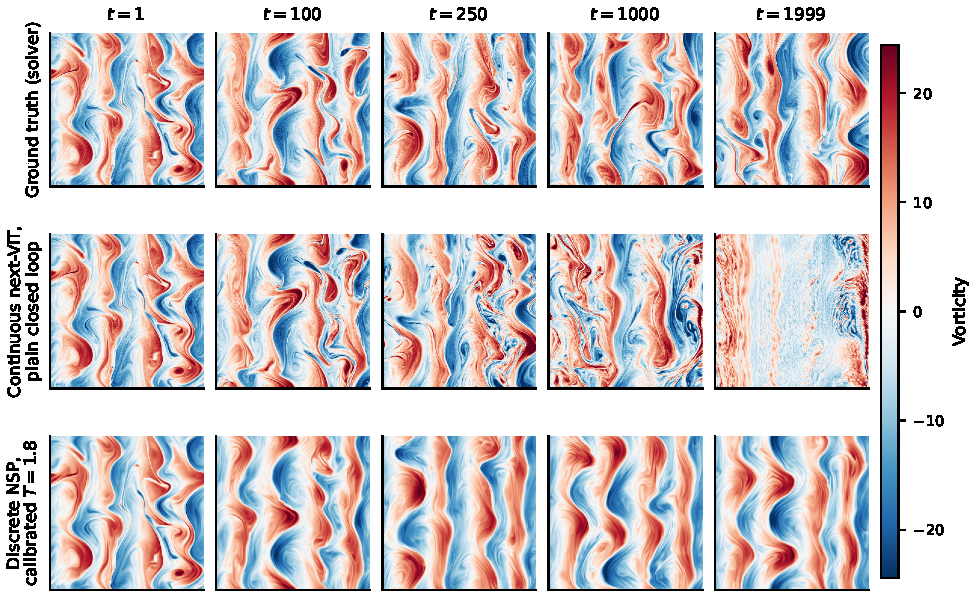
\includegraphics[width=\linewidth]{headline/fig1_offmanifold_rows}
\caption{The long rollout problem. Each row shows a model rollout across time. The continuous ViT baseline model tracks ground truth well but becomes visibly unstable by step 250. The calibrated discrete rollout loses the trajectory but holds the statistical properties until the end of the timeline.}
\label{fig:offmanifold}
\end{figure}

The standard fixes in the literature involve adding different types of stabilizing margins to the network: noise injected into the
training inputs so the model learns to damp the perturbations its own errors will supply \citep{stachenfeld2022learned}; training unrolled through the 
model's own predictions so it optimizes against its own drift, the ``pushforward'' trick \citep{brandstetter2022mppde}; a learned per-step refinement 
that re-amplifies the high-frequency content each step loses \citep{lippe2023pderefiner}; score-based steering of each step back toward the data distribution
\citep{thermalizer2025}. Each of these fixes involves a training-time hyperparameter, and the only way to learn whether or not it is properly tuned is to run the long rollout and score it against ground truth.

The nature of autoregressive instability motivates a shift from regression to classification. If the problem is converted to one of predicting discrete classes, then the
set of outputs (and therefore inputs) is finite and bounded. It is not possible for a classifier to predict a class not in the training data. The challenge is then to find
a way to convert a continuous regression problem into one of classification, which guides our approach.

Our first contribution is the discretized surrogate model: a multi-scale VQ tokenizer and a next-scale-prediction transformer (Section~\ref{sec:method}).
We show that the conversion to discrete tokens does not by itself make the rollout stable; it introduces two different failure modes, and the choice of sampling method controls which one occurs.
Sampling with low entropy (greedy or low temperature) causes the solution to collapse to smooth banded modes. Conversely, sampling with too much entropy (high temperature) 
produces accurate kinetic energy profiles but distorts the vorticity distribution (Section~\ref{sec:greedy}). This has shifted the problem of hyperparameter tuning from training time to test time, 
and the naive method for choosing an optimal temperature is no different from prior architectures: run long rollouts at different temperatures and score them against the ground truth.

This motivates our next contribution: a calibration method that is substantially cheaper than generating many long rollouts and scoring them against ground truth. We develop 
a marginal-entropy calibration that uses training data and short rollouts without ground truth to find the stabilizing sampling temperature needed for long-term rollouts 
(Section~\ref{sec:calibration}). Finally, we compare our results to existing baselines and show that the calibrated discrete rollout's long-run statistics concentrate with window length while
a pushforward-stabilized continuous baseline's do not (Section~\ref{sec:baselines}).


% =====================================================================
\section{Related work}
\label{sec:related}


Neural surrogates for PDEs are most commonly trained as autoregressive regression models
over continuous fields, from convolutional models to spectral operator families
\citep{kochkov2021machine,li2021fourier}. The stabilizing margins developed for these
models are described in the introduction. Work closest to ours extends this paradigm with multi-physics pretraining of autoregressive surrogates
\citep{mccabe2024mpp} and autoregression over continuous latent codes
\citep{serrano2024aroma}. In all of these, the correction is chosen per system and applied
at every rollout step, and the margin a new system needs is discovered only by rolling it
out.

Time series forecasting has also discretized the value axis, gaining access to the
language-model toolbox: a fixed vocabulary, cross-entropy training, and mature sampling
machinery. Digit tokenization puts scalar series directly into a frozen LLM
\citep{gruver2023llmtime}, Chronos builds a quantized value vocabulary and trains on it
\citep{ansari2024chronos}, and TOTEM learns VQ token embeddings \citep{talukder2024totem}.
These models are judged on forecast skill over scalar series; spatial fields and the
statistics of long free-running generation are outside their scope.

The tools for tokenizing spatial fields come from image generation. VQ-VAE and VQGAN turn
images into sequences of tokens drawn from a learned codebook
\citep{oord2017neural,esser2021taming}, RQ-VAE stacks residual codes under an
autoregressive transformer \citep{lee2022rqvae}, and VAR moves the autoregressive axis
from raster order to a coarse-to-fine sequence of scales \citep{tian2024var}. We adopt
VAR's scale interface for our tokenizer (Section~\ref{sec:method}). These generators are
judged on the perceptual quality of single samples, and there is no notion of the
stationary statistics of a generated series.

Closest to this work is a small literature on PDE tokenization: in-context and
foundation-model prediction over discrete PDE tokens \citep{serrano2024zebra,
nguyen2025physix}, and VQ compression of turbulence fields \citep{momenifar2021dimension}.
None of these study stability over multi-thousand-step rollouts, and none calibrate the
sampling distribution.

% =====================================================================
\section{The System}
\label{sec:contlineage}
\label{sec:contchallenge}
\label{sec:system}

Our system of choice is 2D forced turbulence on a $\beta$-plane at $Re = 10{,}000$, evolved in
vorticity form on a doubly periodic $[0, 2\pi]^2$ domain:
      \[
      \frac{\partial \omega}{\partial t} + \mathbf{u} \cdot \nabla \omega + \beta v
        = \frac{1}{Re} \nabla^2 \omega - \alpha\,\omega + F(x, y),
      \qquad
      \omega = \nabla^2 \psi, \quad \mathbf{u} = (-\partial_y \psi,\, \partial_x \psi),
      \]
      with Coriolis parameter $\beta = 20$, Rayleigh drag $\alpha = 0.1$ removing energy at
      the largest scales, and stationary forcing $F = 4(\cos 4x + \cos 4y)$ injecting it at
      wavenumber 4 on both axes.
 We generate our data with a pseudo-spectral solver at $256^2$ with $3/2$-rule dealiasing,
 second-order Adams--Bashforth convection with Crank--Nicolson (implicit) diffusion and drag, at $\Delta t_{\mathrm{solver}} = 10^{-4}$, initialized from a spun-up
 turbulent state so the record is statistically steady throughout. 
      
Each data frame is a vorticity snapshot saved every 100 solver steps ($\Delta t = 0.01$ time units), normalized to zero mean and unit variance. One step
of the surrogate spans what 100 solver steps produce. The training record is ${\sim}20$k consecutive frames (200 time units), with the following 2{,}000 reserved for validation
and rollout initial conditions.


Rollouts are evaluated on the long-run TKE spectrum, computed from the rollout's vorticity frames using the following procedure: invert each frame's vorticity for the streamfunction
($\hat{\psi} = \hat{\omega}/|k|^2$), form the velocities
($\hat{u} = i k_y \hat{\psi}$, $\hat{v} = -i k_x \hat{\psi}$), take the
kinetic-energy spectral density $\tfrac{1}{2}(|\hat{u}|^2 + |\hat{v}|^2)$, average it
over annular shells in $|k|$ (128 linear bins) to get $E(k)$, and average $E(k)$
over every frame of the rollout. The enstrophy spectrum
$Z(k) = \tfrac{1}{2}|\hat{\omega}|^2$ uses the same shells. The reference for both is the
same time average over the held-out data window.


Alongside the spectra we report the pixel vorticity distribution (as an earth mover's
distance, EMD, against the data's), decoded snapshots, and token-space drift;
Section~\ref{sec:metrics} explains why no single one of these is sufficient to diagnose rollout instability. Forecast
skill and long-run statistical fidelity are different objectives with different
optima on this system (Appendix~\ref{app:secondary}).
Figure~\ref{fig:offmanifold} shows the failure this paper addresses, on this system:
the same ViT autoencoder our tokenizer uses, wired instead as a continuous next-frame
regressor and rolled for 2{,}000 steps, leaves the manifold within a few hundred
steps even though its one-step spectrum is essentially exact. The stabilized variants
and the quantitative comparison are in Section~\ref{sec:baselines}.


% =====================================================================
\section{Methodology}
\label{sec:method}
\label{sec:discreteroute}
\label{sec:whydiscrete}

% SCRIPT REGISTER. Recut 07-21 (user): the Tokenization subsection and "Why discrete, why
% a scale axis" are dissolved into this section — the method is justified as it is
% presented. Opening block = why discrete and why learned; the scale-axis case (cost +
% instrument + M6) closes the NSP subsection. Architecture is inherited (VAR) and kept
% brief; details in Appendices~\ref{app:tokenizer} and \ref{app:mask}. The mask stays a
% design-choice line in the NSP subsection; M3 is not a claim of the paper. The old
% sec:discreteroute/sec:whydiscrete labels are carried on this section so existing
% references resolve.

The naive discretization strategy used by Chronos works well in 1D systems, but PDEs are often extremely high-dimensional.
This high dimensionality makes direct value binning of each point in a single timestep nonviable. For our dataset, one token
per grid cell gives 65{,}536 tokens per frame at $256^2$. This would explode to 16{,}777{,}216 at $256^3$, so we must learn a
compressed discretization. Rather than specify one, we turn to the image generation literature and borrow its techniques to learn one.
A learned discretization has the benefit of bounding the state by construction: every token sequence decodes to a field in the decoder's range,
making value blow-up impossible.

Beyond boundedness, tokens offer other advantages. The training data's token statistics form a reference distribution (Section~\ref{sec:calibmethod}).
Failures therefore become measurable events during a rollout: an emitted token the training set never placed at that position, or an emitted token
distribution measurably narrower than the data's (Section~\ref{sec:greedy}). Additionally, a well-calibrated rollout's long-run statistics will
concentrate with window length (Section~\ref{sec:baselines}).

It is worth emphasizing that despite being bounded, tokenization by itself stabilizes nothing. While the solution will stay bounded, the long-run statistics
can still diverge despite every emitted token being legal at its position (Section~\ref{sec:greedy}). Stability instead comes from the sampling distribution.

\subsection{Multi-scale tokenizer}
\label{sec:tokenizer}

We adopt VAR's scale interface for the learned discretization. A ViT autoencoder with a
strided-conv stem maps the $(1,256,256)$ vorticity field to a $(512,32,32)$ latent, and a
multi-scale residual VQ quantizes that latent against a single shared EMA codebook
($K{=}4096$, $d{=}512$): quantize at $1{\times}1$, upsample, quantize the residual, and
repeat up to $32{\times}32$ (Figure~\ref{fig:arch}). The codebook holds a $256^2$ frame in
341--1{,}941 tokens, a compression rate of $34$--$192{\times}$ in 2D. We name tokenizers by
their token budget per frame: sc341, sc917, and sc1941.

Quantization is a deterministic argmax over the codebook, which removes a sampling knob
from the tokenizer at a cost to high-wavenumber performance; Figure~\ref{fig:reconrow}
shows the loss in accuracy. Because the learned tokens encode local flow patterns rather
than value bins, per-scale token statistics correspond to physical properties of the
field, and because tokens decode through a fixed deterministic map, any token statistic
converts to a field statistic through a single pushforward.

The scale structure itself does not improve reconstruction: flat single-scale control
tokenizers at matched budget reach the same reconstruction floor (flat-1024 reaches EMD
0.108 against sc917's 0.107, Table~\ref{tab:reconfloor}), so reconstruction quality is set
by token count. The case for the scale axis is made at the end of Section~\ref{sec:nsp}. We
take the error from the tokenizer as a fixed cost, referred to as the model's floor, and 
all discrete rollout spectra are compared against it.


\begin{figure}[!htb]
\centering
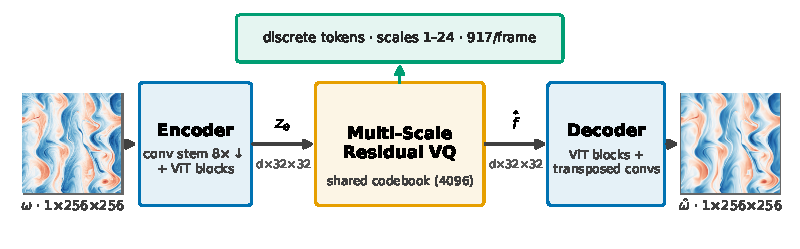
\includegraphics[width=0.82\linewidth]{vqvae_arch}\\[6pt]
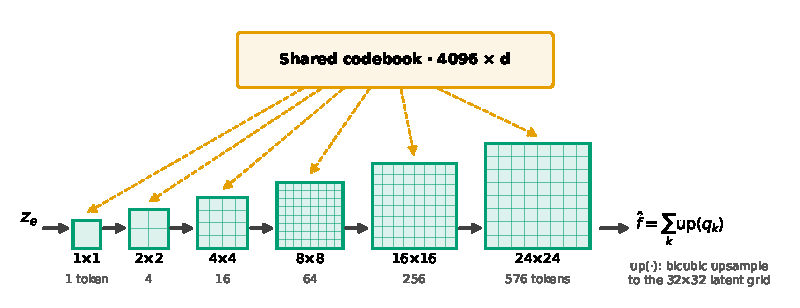
\includegraphics[width=0.82\linewidth]{multiscale_vq}
\caption{The tokenizer. The ViT autoencoder (top) and the multi-scale residual VQ loop with
the shared codebook (bottom).}
\label{fig:arch}
\end{figure}

\begin{figure}[!htb]
\centering
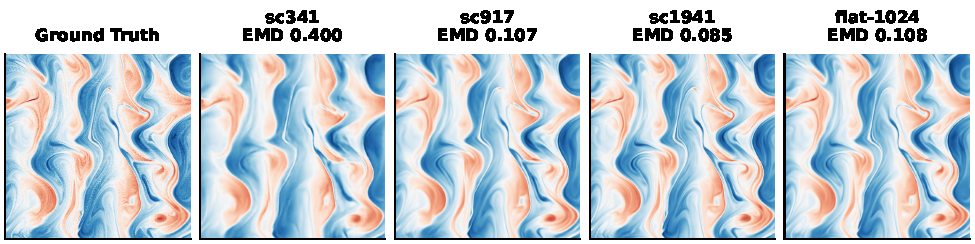
\includegraphics[width=\linewidth]{recon_floor/arch_recon_row}
\caption{Ground truth and its
reconstruction through each tokenizer with average EMD floor.}
\label{fig:reconrow}
\end{figure}

\subsection{Next-scale prediction model}
\label{sec:nsp}

The dynamics model is a VAR-style transformer (RMSNorm, QK-norm, bias-free projections,
SwiGLU, 2D axial RoPE on cell-center coordinates) that predicts scale $k$ of frame $t{+}1$
from scale $k{-}1$'s hidden states through a shared refinement stack. Attention follows a
prefix-LM pattern: full attention toward the conditioning frame, block-causal within the
target (Figure~\ref{fig:nsp}).
% This is the abstract's "prefix-LM-style" claim.
Emitting an entire scale each forward pass significantly reduces the cost of long
rollouts. Raster-order autoregression emits one token per sequential pass, so 1024 tokens per frame
means ${\sim}2.05$M sequential passes for a 2{,}000-step rollout; next-scale prediction
takes ${\sim}12$k passes for sc917 (one per scale; 10--14k across the three families),
within ${\sim}6{\times}$ of the $2$k passes of flat one-shot or continuous per-frame
prediction (one per frame). The passes differ in width: a raster pass emits one token, an
NSP pass a whole scale.
% fig:cost CUT 08-25 (user: a bar chart of three numbers). The numbers live in the
% sentence above; the sec:baselines cost paragraph back-references sec:nsp.
Training minimizes per-scale cross-entropy weighted by $1/\log(n_k{+}1)$, and
teacher-forced inputs receive 10\% token-substitution noise, a discrete analogue of
pushforward-style input perturbation \citep{brandstetter2022mppde,stachenfeld2022learned}.
At rollout time each emission is masked to the tokens the training set has at
that exact position. A per-scale variant, which allowed any valid token within the entire scale, led to token combinations never seen by the decoder, which can decode to high-frequency static, so we mask per position. Rollout outcomes are set by the sampling distribution
(Section~\ref{sec:greedy}); the granularity ablation is in Appendix~\ref{app:mask}.

Our addition of scales is primarily motivated by sampling calibration. A single-scale flat-1024 token model can hold a 2{,}000-step rollout. When we swept across temperatures, we found that at $T{=}1.6$ both flat NSP models run the full horizon essentially at their tokenizer floor (EMD 0.115/0.126 against
0.108). They still fail cold and hot in the same ways our multi-scale approach does
(Appendix~\ref{app:secondary}, Figure~\ref{fig:flatnsp}), and the scale decomposition enables additional diagnostic instruments: a per-scale token readout that provides a stabilization
method. Because entropy drains fastest at the fine scales (Section~\ref{sec:greedy}), the
per-scale entropy profile is a calibration target. Instead of sweeping the temperature
with expensive rollouts, we can solve for it from the entropy of the finest scales (Section~\ref{sec:calibration},
Figure~\ref{fig:schedule}). Coarse scales also cost almost nothing in the residual stack,
whereas refining a flat tokenizer means growing its single grid quadratically.
Tokenization has so far provided detection and a diagnostic axis but no stability without an expensive temperature sweep across rollouts; the
next section develops the calibration enabling that.

\begin{figure}[!htb]
\centering
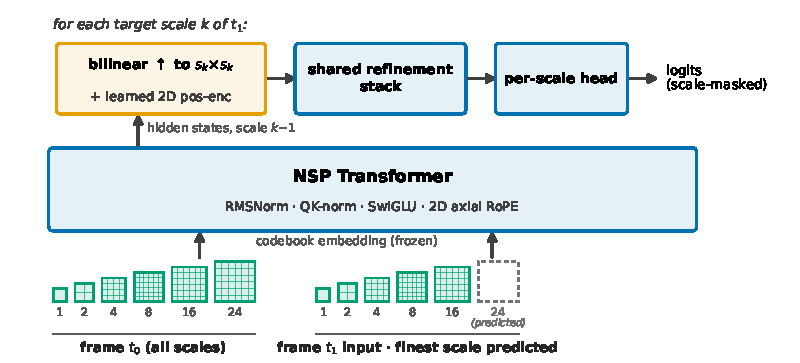
\includegraphics[width=0.82\linewidth]{nsp_arch}\\[6pt]
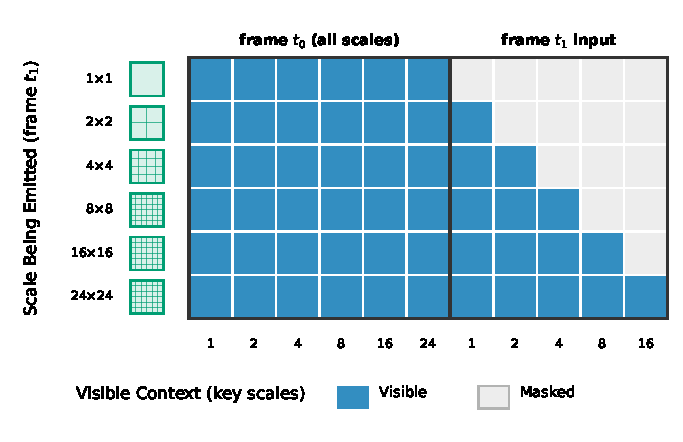
\includegraphics[width=0.7\linewidth]{attention_mask}
\caption{The NSP model. The backbone with expansion heads and shared refinement (top) and the
asymmetric [full $t_0$, truncated $t_1$] attention mask (bottom).}
\label{fig:nsp}
\end{figure}

% =====================================================================
\section{Marginal-entropy calibration}
\label{sec:calibration}

\subsection{The discrete failure modes}
\label{sec:greedy}

Unlike the continuous baseline of Figure~\ref{fig:offmanifold}, discrete rollouts can fail without any overt signal. Greedy decoding, the natural default for a discrete surrogate,
can lose fine structure within ${\sim}100$ steps for large-token-count architectures and settle into smooth large-scale banding
while the tokenizer reconstruction at the same lead time remains indistinguishable from
ground truth (Figure~\ref{fig:failuremodes}, center).

Raising the temperature fails in the opposite direction. Heating the fine scales to $T{=}4.0$ turns the field fuzzy, 
but it returns the spectrum exactly to the tokenizer-reconstruction curve and improves every scalar metric over the
collapsed arm: TKE error $0.60$ against $0.88$ and EMD $0.45$ against $0.79$, from a
\emph{smaller} model (Figure~\ref{fig:failuremodes}, right). Only examining the pixel distribution
and the field itself reveals the failure (Section~\ref{sec:metrics}).

Greedy decoding is a $T{\to}0$ limit, cold
finite sampling at $T{=}0.7$ collapses the same way, and Figure~\ref{fig:failuremodes}
shows what these failure modes look like. A calibration method must therefore
determine what to set the temperature to and against what reference. 

The per-scale token readout of Section~\ref{sec:method} shows that the emitted tokens exhibit entropy draining at every scale
and fastest at the fine ones (Figure~
ef{fig:modeb}), while every token stays individually legal: the joint
distribution has drifted to the smoothest corner of the support. We use the
training data's per-scale token entropy as a reference line for both the diagnosis of failed rollouts and the target for successful ones. The goal of a calibrated sampler is to emit at the data's entropy level on the finest scales, where the drain is fastest. A flat tokenizer or a continuous field has no analogous readout.

The calibration must target a horizon statistic because
$H(X_k) = H(X_k \mid \mathrm{past}) + I(X_k;\mathrm{past})$. At coarse scales the
conditional term is near zero, so the long-run diversity lives in the temporal
term, which no single-step statistic can measure. The collapse consists of the rollout's
marginal falling below the data's while every conditional stays accurate. Only the
emitted-token marginal aggregated over a free-running horizon can capture this.

\begin{figure}[!htb]
\centering
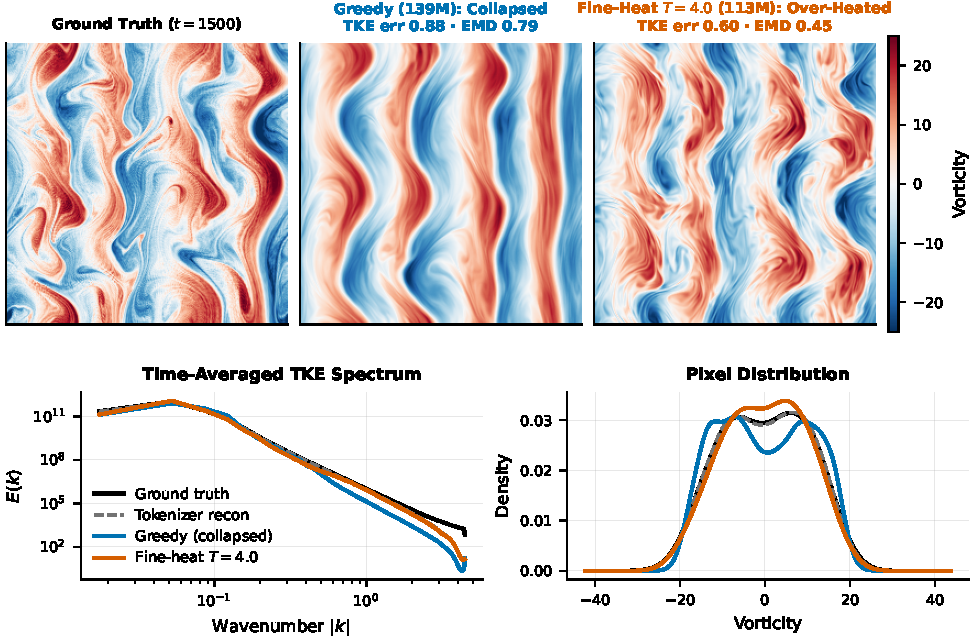
\includegraphics[width=\linewidth]{mode_diagnostics/failure_modes_pair}
\caption{Top, left to right: ground truth at $t{=}1500$; greedy
decoding collapsed into smooth banding (139M NSP); fine scales over-heated at
$T{=}4.0$ turned fuzzy (113M NSP). Bottom: time-averaged TKE spectra and pixel distributions
over the full 2{,}000-step rollouts ($N{=}1$ and $N{=}128$ trajectories respectively). 
Scalar measures incorrectly rate the over-heated arm the highest, while its error can be clearly seen in the distribution.}
\label{fig:failuremodes}
\end{figure}

\begin{figure}[!htb]
\centering
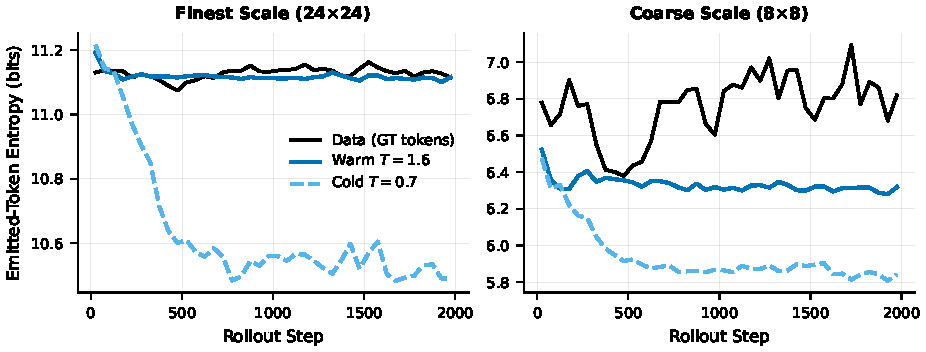
\includegraphics[width=0.95\linewidth]{mode_diagnostics/mode_b_entropy_cliff}
\caption{Comparison of collapsed trajectories versus ground truth in token space.
Emitted-token entropy per window (sc917, 16 trajectories) against the entropy of the ground-truth tokens at the same positions. Cold sampling drains entropy at every scale, fastest at the finest; warm sampling stays at the data's entropy for 2{,}000 steps, but only at the finest scale. 
}
\label{fig:modeb}
\end{figure}

\subsection{Calibration method}
\label{sec:calibmethod}

Both failure modes of Section~\ref{sec:greedy} are entropy imbalances. Sampling too hot
injects entropy the system does not have, and sampling too cold drains entropy it does.
We looked to answer whether the sampler can be calibrated to the data's entropy
without an expensive sweep over sampling hyperparameters. Because the statistics of our system are stationary in expectation, the data's token entropy is a fixed target that any model can be matched to. The goal of our calibration is to find a sampling
method that keeps rollouts out of both failure modes over the whole horizon, which is not necessarily the rollout with the lowest EMD or TKE spectral error.

Section~\ref{sec:greedy} already found the statistic to match, the emitted-token marginal aggregated over a free-running horizon. Stationarity also removes the problem of finding the window length. Because the windowed statistic converges as the window grows, window size is
not a hyperparameter (this was measured as train-vs-val excess JS
$\leq 1.5{\times}10^{-2}$ bits across all nine tokenizers). The
teacher-forced single-step alternative is compared below.

The calibration has three steps. Step (1) computes the target: the per-scale marginal
token entropy $H^{\mathrm{data}}_k$ of the tokenized training set. The target reflects the physics of the system (Figure~\ref{fig:entropytarget}). In every
tokenizer family, the finest scales have the highest entropy, consistent with turbulence
concentrating its diversity in the small scales, and the profile is close to linear in the log of the scale resolution. It is also a property of the tokenizer family and not of the autoencoder size, since the three VQ sizes overlay.

\begin{figure}[!htb]
\centering
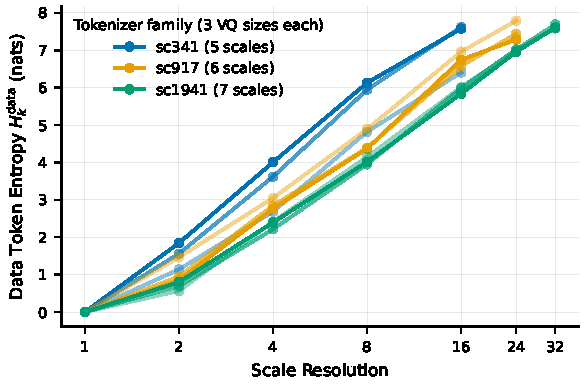
\includegraphics[width=0.6\linewidth]{per_scale_temp/entropy_profile}
\caption{The calibration target from step (1). The per-scale marginal token entropy of the tokenized training set for all nine tokenizer configurations (three VQ sizes overlaid per family). The finest scales have the highest entropy, close to linear in log resolution; the profile is a property of the tokenizer family, not the autoencoder size.
}
\label{fig:entropytarget}
\end{figure}

Step (2) measures the response: the rollout's horizon-aggregated emitted-token marginal
entropy $H^{\mathrm{roll}}_k(T)$. The response is a property of the model's closed loop
rather than the tokenizer's (models sharing a tokenizer solve to temperatures spanning
0.3 on sc917 to 1.6 on sc341 across our grid), so it is measured per model from
diagnostic rollouts. A diagnostic rollout is one free-running trajectory scored on its
own emitted tokens. The first probe runs at $T{=}1$, the sign of the measured gap $H^{\mathrm{roll}}_k(1) - H^{\mathrm{data}}_k$ on the finest scales sets the search direction, and subsequent probes step outward until the gap changes sign, which brackets the crossing. Every response curve we measured is monotone in $T$ up to sampling noise (removed by a running maximum before inverting), so two bracketing probes determine the solution. Step (3) solves for one global
temperature $T^\ast$: every scale is sampled at the same $T$, and $T^\ast$ is the zero of
the averaged gap on the finest two scales $\mathcal{F}$, the scales that drive the
collapse, found by linear interpolation inside the bracket:
\begin{equation}
g(T) \;=\; \tfrac{1}{2}\textstyle\sum_{k\in\mathcal{F}}
\big[H^{\mathrm{roll}}_k(T) - H^{\mathrm{data}}_k\big] \;=\; 0
\qquad \text{(all scales sampled at $T$)}.
\label{eq:globalread}
\end{equation}
The coarse scales are sampled at $T^\ast$ too; only the finest two enter the solve. The
solve reads tokens only, and EMD and spectra enter at evaluation time
(Section~\ref{sec:experiments}). We call the solved temperature $T^\ast$ the read, since
it is read from tokens. We deploy the read against $N{=}128$ sweeps across all
45 (model, tokenizer) cells, with the response curves read off the sweep's own rollouts,
and end to end on five cells with fresh diagnostic rollouts. A per-scale temperature, one
$T_k$ per scale, is discussed as future work (Appendix~\ref{app:future}).

We tested the calibration end to end on five cells: two on sc917, two on sc1941, and one
on sc341, covering the three VQ sizes. On each cell we start at $T{=}1$; the sign of $g(T)$
(Equation~\ref{eq:globalread}) sets the direction, positive meaning the rollout emits more
fine-scale entropy than the data and the temperature must fall, and we step by 0.2 in
that direction until $g$ changes sign, then interpolate the zero crossing between the two
bracketing temperatures. Temperature calibration required one rollout of 250 steps on sc917 and sc1941 and four rollouts of 250 steps on sc341. The five cells bracketed within five to eight temperatures each
(Table~\ref{tab:deploy}).

On every cell the calibrated temperature lands within 0.05 of the same solve run on the
full sweep's rollouts, 128 trajectories of 2{,}000 steps: 0.005 to 0.048. We then rolled
each calibrated temperature out at $N{=}128$ for 2{,}000 steps and scored it against
ground truth. EMD is 0.003 to 0.131 above the sweep's minimum on the four sc917 and
sc1941 cells and 0.414 above it on the sc341 cell. The 0.414 is not a precision failure,
since that cell's calibrated temperature is within 0.048 of the full solve. sc341 has no
cold failure for the calibration to prevent (Figure~\ref{fig:global341}), so the extra
warmth only raises EMD.

We measured how short the diagnostic rollouts can be on all 45 cells by truncating and
subsetting the sweep's own rollouts and solving from the truncated marginals
(Figure~\ref{fig:diagmulticell}). Against the full solve, one trajectory of 250 steps
lands within 0.05 on all 30 sc917 and sc1941 cells, and 96\% and 99.8\% of the
individual draws land within 0.05. On sc341, one trajectory of 250 steps lands above
the full solve, by 0.135 on the median cell and 0.42 on the worst, and 21\% of draws
land within 0.05. Four trajectories of 250 steps bring the median cell to 0.035 above,
with 66\% of draws within 0.05; one trajectory of 1{,}000 steps brings it to 0.037, with
70\%; four trajectories of 1{,}000 steps reach 97.5\%. sc341 needs the extra trajectories
because its response is flat: 0.13 nats per unit of $T$ on its finest two scales against
0.45 on sc917 and 0.62 on sc1941, so the same entropy error is a 3.5 to 5 times larger
temperature error.

The calibration uses training tokens and the model's own emitted tokens during rollout.
In comparison, a rollout sweep needs many long-run ground-truth references to score against.
The calibration generates 1{,}250 to 2{,}000 frames per cell on sc917 and sc1941 and
8{,}000 on sc341, scored as token histograms without requiring decoding into pixels. The $N{=}128$ sweep
required decoding and scoring 1.28M frames per cell.

\begin{figure}[!htb]
\centering
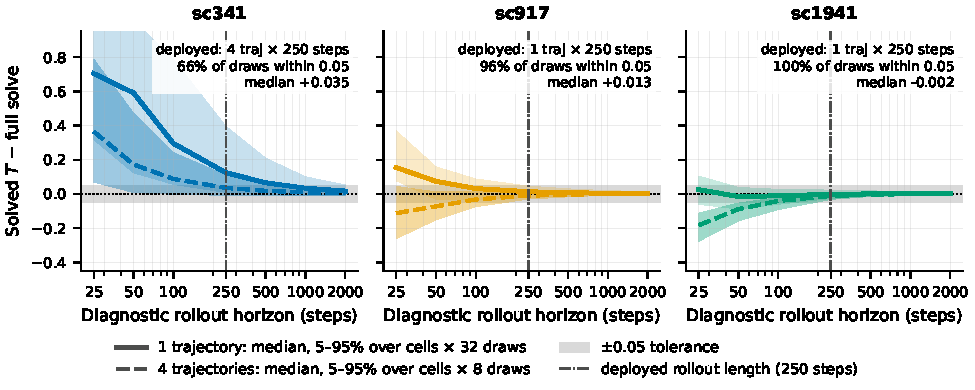
\includegraphics[width=\linewidth]{diag_multicell/convergence_signed}
\caption{The cost of the calibration, validated on all 45 cells. Each panel shows the signed
deviation of the truncated solve from the full 128-trajectory, 2{,}000-step solve against
the diagnostic horizon for one family. The line is the median and the band is the 5--95\%
range over cells and draws (32 single-trajectory draws or 8 four-trajectory draws per
cell), the gray band is the $\pm 0.05$ tolerance, and the dash-dot line is the deployed
rollout length of 250 steps. A single trajectory is warm at short horizons and a pooled
marginal is cold on sc917 and sc1941, and both close by 250 steps. One trajectory of 250
steps is enough on sc917 and sc1941, and sc341's flatter response needs four.}
\label{fig:diagmulticell}
\end{figure}

\begin{table}[!htb]
\centering\small
\caption{End-to-end deployments of the calibration on five cells. Each temperature is scored by
one 250-step rollout (four on sc341), starting from $T{=}1$ and stepping by 0.2 in the
direction of the gap's sign, and $T^\ast$ is the zero crossing interpolated between the two
bracketing temperatures. EMD is the $N{=}128$, 2{,}000-step evaluation at $T^\ast$ against
ground truth, the swept argmin and its EMD come from the $N{=}128$ sweep, and regret is
their difference. The validation sweep cost 1.28M decoded frames per cell.}
\begin{tabular}{lrrrrrr}
\toprule
cell & temperatures & frames & $T^\ast$ & EMD & swept argmin (EMD) & regret \\
\midrule
medium-sc917-s34 & 6 & 1{,}500 & 1.873 & 0.250 & 1.6 (0.119) & 0.131 \\
small-sc917-s22 & 6 & 1{,}500 & 1.868 & 0.196 & 1.8 (0.187) & 0.009 \\
large-sc1941-s48 & 5 & 1{,}250 & 1.742 & 0.217 & 1.4 (0.157) & 0.060 \\
medium-sc1941-s113 & 8 & 2{,}000 & 2.211 & 0.144 & 2.2 (0.141) & 0.003 \\
medium-sc341-s18 & 8 & 8{,}000 & 2.345 & 0.547 & 1.2 (0.133) & 0.414 \\
\bottomrule
\end{tabular}
\label{tab:deploy}
\end{table}

We tested the single-step alternative in both its forms, and both fail. The strongest
anchor solves
$H(\mathrm{softmax}(z_k/T_k)) = \mathrm{CE}_k$ per scale on teacher-forced
logits\label{sec:gate}, since overconfidence is the textbook cause of degenerate
free-running generation. However, the measured gap $\mathrm{CE}-H$ is at or below zero at
every scale ($-0.09$ to $-0.32$ nats at the finest), so the solved temperatures never leave
$T\leq 1$ while swept optima on warm configurations sit at 1.8--2.2. Teacher forcing holds
the model on the data manifold, where it is calibrated; the extra warmth compensates for
what happens off the manifold, which no teacher-forced statistic measures
(Appendix~\ref{app:secondary}, Figure~\ref{fig:calibgate}). 

We also compare against the brute-force alternative of sweeping temperature per cell at
$N{=}128$, on the 15-cell sc1941 grid (Figure~\ref{fig:schedule}; sc917/sc341 analogs in
Appendix~\ref{app:secondary}, Figures~\ref{fig:global917},~\ref{fig:global341}). Greedy
decoding is erratic, fine on some cells and exploding on others (EMD $0.19$--$5.6$, above
our explosion threshold of EMD 1.0 on 4 of 15 cells). The cold sweep edge, $T{=}1.4$, is above
the swept optimum, the swept temperature with the lowest ensemble EMD on the cell, by a
median 0.27 EMD, explodes on 3 cells, and has the largest spectral error of
the sampled arms on 14 of 15, the spectral drain of Section~\ref{sec:greedy}. The hot
edge, $T{=}2.2$, has the lowest spectral error on 7 of 15 cells and is above the optimum
by a median 0.30 EMD, the over-heat failure of Figure~\ref{fig:failuremodes}, where the
spectrum improves while the pixel distribution degrades. The read temperature, rounded
to the nearest swept temperature, explodes nowhere and is above the optimum by a median
0.11 EMD: it is the only sampled arm with EMD under 1.0 on every cell, and it does not
reach the swept optimum (Section~\ref{sec:limitations}).

We then deployed the read as one global temperature against the $N{=}128$ sweeps on all
45 cells, solving against the training-set token entropy of step (1). In every cell the
sweep brackets the solved temperature, with a swept point on each side of it. On 13 cells the gap $g(T)$ was still negative at the original sweep's
hottest temperature, so we extended the sweep by two hotter temperatures on those cells
(2.4 and 2.8 on sc917, 2.6 and 3.0 on sc1941) until it bracketed the solved temperature.

\begin{table}[!htb]
\centering\small
\caption{The read against the $N{=}128$ sweep, by tokenizer family (15 cells each). A read is
inside the interval when both swept temperatures bracketing it have an ensemble EMD under the
bar. The regret is the ensemble EMD at the read, interpolated between the bracketing swept
temperatures, minus the ensemble EMD at the swept argmin, both at 2{,}000 steps against ground
truth. The count of 42 does not change under trajectory resampling, since the standard error of
the ensemble EMD is at most 0.005 at every bracketing temperature. The read is inside the
interval on 42 of the 45 cells and warmer than the argmin on 43, and the median regret is 0.19
EMD.}
\newcommand{\hdr}[1]{\begin{tabular}[c]{@{}c@{}}#1\end{tabular}}
\begin{tabular}{lcccccc}
\toprule
family & \hdr{inside the interval\\bar 1.0 / 0.75 / 0.5} & \hdr{read $-$ argmin\\median $\Delta T$} & \hdr{warmer /\\colder} & \hdr{regret\\median (IQR)} & \hdr{regret\\$\leq 0.1$ / $\leq 0.2$} & \hdr{max\\regret} \\
\midrule
sc341  & 15 / 12 / 2  & $+1.03$ & 15 / 0 & 0.26 (0.20--0.37) & 0 / 4   & 0.49 \\
sc917  & 15 / 14 / 10 & $+0.15$ & 13 / 2 & 0.14 (0.04--0.19) & 7 / 12  & 0.51 \\
sc1941 & 12 / 9 / 7   & $+0.25$ & 15 / 0 & 0.13 (0.08--0.32) & 7 / 8   & 0.61 \\
\midrule
all    & 42 / 35 / 19 & $+0.34$ & 43 / 2 & 0.19 (0.09--0.32) & 14 / 24 & 0.61 \\
\bottomrule
\end{tabular}
\label{tab:outcome}
\end{table}

Table~\ref{tab:outcome} compares the read with the $N{=}128$ sweep on all 45 cells. In 42 of
the 45 cells the read lies inside the non-exploded interval, the set of swept temperatures at
which the ensemble EMD against ground truth stays under 1.0. The three cells outside it are
sc1941 cells whose read falls between the hottest non-exploded swept temperature, 2.2, and the
first exploded one, 2.6. We deployed one of them, medium-sc1941-s113, in
Table~\ref{tab:deploy}, and it scored an EMD of 0.144. The other two are the 31M-parameter
models under the small and medium VQ, and their EMD interpolated between the two bracketing
sweep points is 0.80 and 0.95. In 43 of the 45 cells the read is warmer than the swept
EMD-argmin, the swept temperature with the lowest ensemble EMD on the cell, by a median of
0.34 in temperature, and on sc341 by 1.03. Because the calibration matches the entropy of the
training data rather than minimizing the EMD, the rollout at the read has a higher EMD than the
rollout at the argmin. We call this difference the regret. Over the 45 cells the median regret
is 0.19 EMD, 0.13 to 0.14 on sc917 and sc1941 and 0.26 on sc341
(Figure~\ref{fig:regret}). On sc341 every rollout at the read stays on-manifold, and the
regret is the EMD increase between the argmin and the warmer read
(Figure~\ref{fig:global341}).

sc341 has no cold failure for the calibration to prevent. Greedy decoding and the cold
sweep edge ($T{=}0.8$) stay on-manifold in 14 of its 15 cells, and on those 14 greedy is
within 0.08 EMD of the swept optimum and the cold edge within 0.12
(Figure~\ref{fig:global341}). The exception is the smallest model with the small VQ, where
greedy and the cold edge score EMD above 0.8 and the read 0.48. On the other 14 cells the
calibration prevents nothing and only adds tail energy at an EMD cost, up to 0.41 on the
deployment cell (0.547 at the read against 0.133 at the argmin). The diagnostic rollouts
that solve for the read also measure the response slope, and the slope identifies this
regime before the read is used: sc341's response slope is 0.13 nats per unit of $T$
against 0.45 and 0.62 on sc917 and sc1941, and on the three families of this paper a flat
response coincides with a cold edge that stays on-manifold and a read with a large regret.
With three families this is an observation and not a validated rule, so we offer the slope
as the indicator to check on a new system before running the rollout at the read's warmer
temperature.

The extra warmth only changes the spectrum in the tail. In the resolved range, the
wavenumbers where the tokenizer floor holds at least half the true energy, the rollout's
energy is at the tokenizer floor both at the swept argmin and at the read (medians 0.95 to 1.09 and 0.98 to 1.03
of floor across the families). In the tail beyond it, energy relative to the floor rises
from 0.60, 0.54, and 0.38 at the argmin to 0.97, 0.67, and 0.50 at the read for sc341,
sc917, and sc1941, at a median regret of 0.26, 0.14, and 0.13 EMD. At the families' cold
edges the tail energy is 0.60, 0.32, and 0.21 of floor (Appendix~\ref{app:secondary},
Figure~\ref{fig:phasediagram}).

\begin{figure}[!htb]
\centering
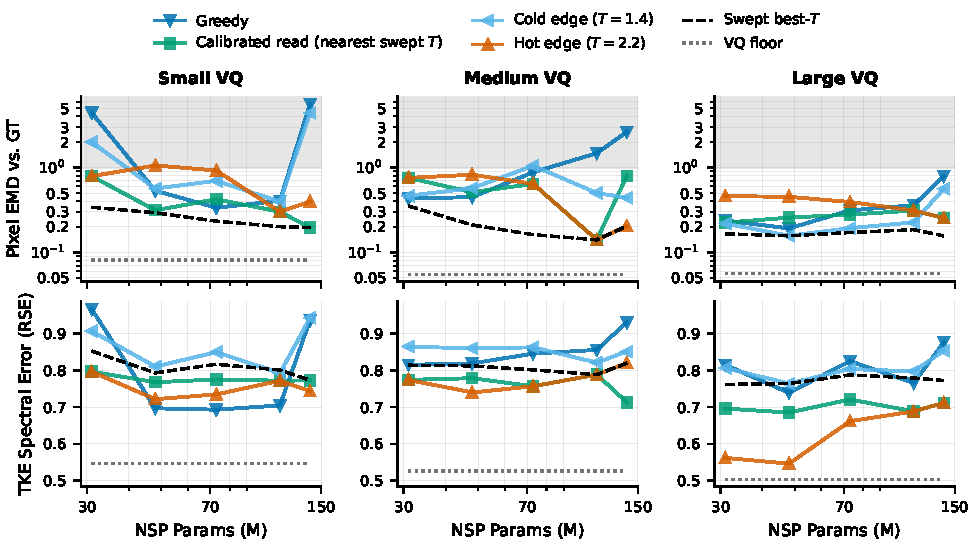
\includegraphics[width=\linewidth]{per_scale_temp/global_outcome_sc1941}
\caption{The temperature axis on the 15-cell sc1941 grid. Pixel EMD (top) and TKE spectral error
(bottom) against NSP size, one column per VQ tier. The arms are greedy decoding ($N{=}1$),
the cold and hot edges of the sweep ($T{=}1.4$ and $2.2$, the range swept on every cell,
$N{=}128$), the calibrated global read rounded to the nearest swept temperature
($N{=}128$), and the swept best-$T$ yardstick (dashed), the swept temperature with the
lowest ensemble EMD on each cell. The two rows have to be read together: the hot edge has the lowest spectral error on the large-VQ column and is the
direction of the fuzzy field of Figure~\ref{fig:failuremodes}, and greedy's low EMD on
some cells is the banded field. The gray band is EMD above the explosion bar of 1.0.}
\label{fig:schedule}
\end{figure}

% =====================================================================
\section{Experiments}
\label{sec:experiments}

All results share one evaluation grid: nine tokenizers (three token budgets
sc341/sc917/sc1941 $\times$ three autoencoder sizes) crossed with five NSP sizes gives 45
(model, tokenizer) cells, and every swept point is an $N{=}128$-trajectory ensemble of
2{,}000-step rollouts. We evaluated each cell at its swept-optimal $T$ ($N{=}128$).

\subsection{Scaling}
\label{sec:scaling}

Long-rollout EMD saturates with NSP size well before the token budget saturates, and 
the tokenizer family sets the maximum attainable band (Figure~\ref{fig:scaling}, right).
Growing the NSP model past medium size does not improve the rollout statistics; growing the token budget does.

The rollout obeys a different scaling law from the single step. Teacher-forced
cross-entropy keeps falling with NSP size, strictly monotone in all nine (family, VQ-tier)
columns and by 22.5--34.4\% from smallest to largest (Figure~\ref{fig:scaling}, left),
while the rollout EMD has already saturated (right) and the rollout's spectral error
worsens with size. With the three shallow-wide architectures included, six of the nine
columns stay monotone. Cross-entropy selects the largest model in every column, and that
model is rollout-best by EMD in three of nine columns and by spectral error in one of
nine. The single-step evaluations cover all
three families with 1{,}999 held-out pairs per cell. As with the continuous baseline
(Section~\ref{sec:baselines}), additional capacity improves next-token accuracy but not
the closed-loop statistics.

\begin{figure}[!htb]
\centering
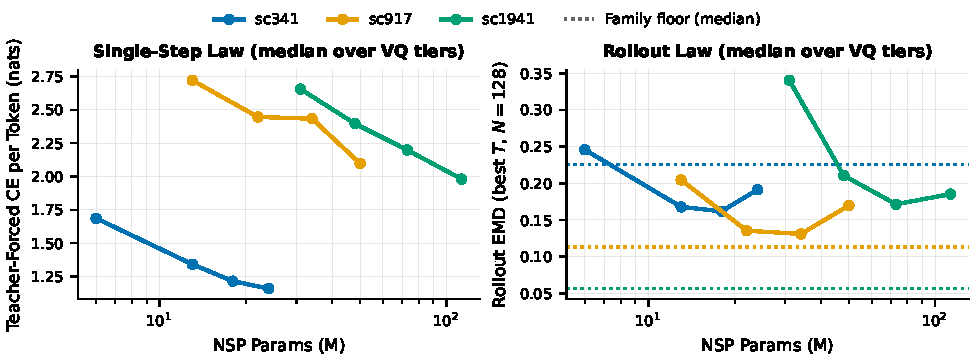
\includegraphics[width=\linewidth]{scaling_n128/scaling_two_laws}
\caption{Two scaling laws. Left: teacher-forced cross-entropy per token improves monotonically with
NSP size in every (family, VQ-tier) column, by 22.5--34.4\% from smallest to largest.
Color is the tokenizer family and shade is the VQ tier. Right: ensemble EMD at each cell's
swept best $T$ ($N{=}128$), median across VQ tiers per family, saturates with NSP size.
The dotted lines are each family's median tokenizer floor, so the token budget and not
the dynamics model sets the attainable band. The shallow-wide architectures are excluded
from both panels.}
\label{fig:scaling}
\end{figure}

\subsection{Metrics}
\label{sec:metrics}

The temperature axis fools each scalar metric in one direction. On the hot side, TKE spectral error improves
monotonically up to $T{=}3.0$ on the sc341 hot edge while EMD triples and the jets lose
coherence. High-$T$ sampling adds energy in exactly the tail the spectrum measure rewards, so a
rollout can improve its spectral error by emitting noise (Figure~\ref{fig:failuremodes}
shows the same effect in a single cell). On the cold side, EMD keeps improving as the
turbulence fades into banding, and the pixel distribution over-sharpens before EMD notices
(Appendix~\ref{app:exhibits}, Figure~\ref{fig:temprows}). Integrated statistics are also
blind to redistribution, since the collapse and the tail deficit both conserve total
energy while moving it across $k$ (measured on our own best model in
Section~\ref{sec:baselines}). % CORRECTION 08-25 (review response): metrics: ΔH is the online proxy for the decoded spectrum, validated against it, not the arbiter

Because of this, we report spectra, distributions, and snapshots together everywhere, and
we use ensembles to adjudicate and individual frames to illustrate. Token-space drift, the
finest-two-scale gap $\Delta H$ between the rollout's emitted-token entropy and the
training-set token entropy, is the online proxy for the spectrum: it is computed from the
emitted tokens during the rollout, with nothing decoded. Across the 326 (cell, $T$) points
of the sweep, the rank correlation of $\Delta H$ with the decoded rollout's tail energy
relative to the tokenizer floor is 0.87, with EMD it is 0.37, and with the energy in the
resolved range it is $-0.02$. The sign of $\Delta H$ detects the spectral drain that EMD
does not see, and the phase diagram
(Appendix~\ref{app:secondary}, Figure~\ref{fig:phasediagram}) colors every sweep point by
the decoded tail retention with the $\Delta H{=}0$ crossing overlaid.

\subsection{Calibrated Rollouts}
\label{sec:perclass}

Figure~\ref{fig:perclass} shows the calibrated rollouts family by family; the spectra and
pixel PDFs of all 45 cells are in Appendix~\ref{app:exhibits} (Figure~\ref{fig:hierarchy}). The best cell of
each tokenizer family is shown at its swept-optimal temperature against its own references. All
three are in the medium VQ tier. The optimal warmth rises with token budget
(swept optimum $T = 1.1 / 1.6 / 2.2$ for sc341/sc917/sc1941), which is the trend predicted by the
calibration. At $t{=}1500$ every field is still fully turbulent, each time-averaged
spectrum sits on its tokenizer-reconstruction curve through the resolved range, and the
pixel distributions sit on the data; the residual high-$k$ gap to ground truth is the
tokenizer floor (Section~
ef{sec:tokenizer}). Ensemble EMD against each
family's floor is $0.14$ vs $0.23$ for sc341, below its own floor by the mode-averaging
effect (Appendix~\ref{app:secondary}); $0.12$ vs $0.11$ for sc917, at floor; and $0.14$ vs
$0.06$ for sc1941, the stationary joint-level residual discussed in
Section~\ref{sec:limitations}.

\begin{figure}[!htb]
\centering
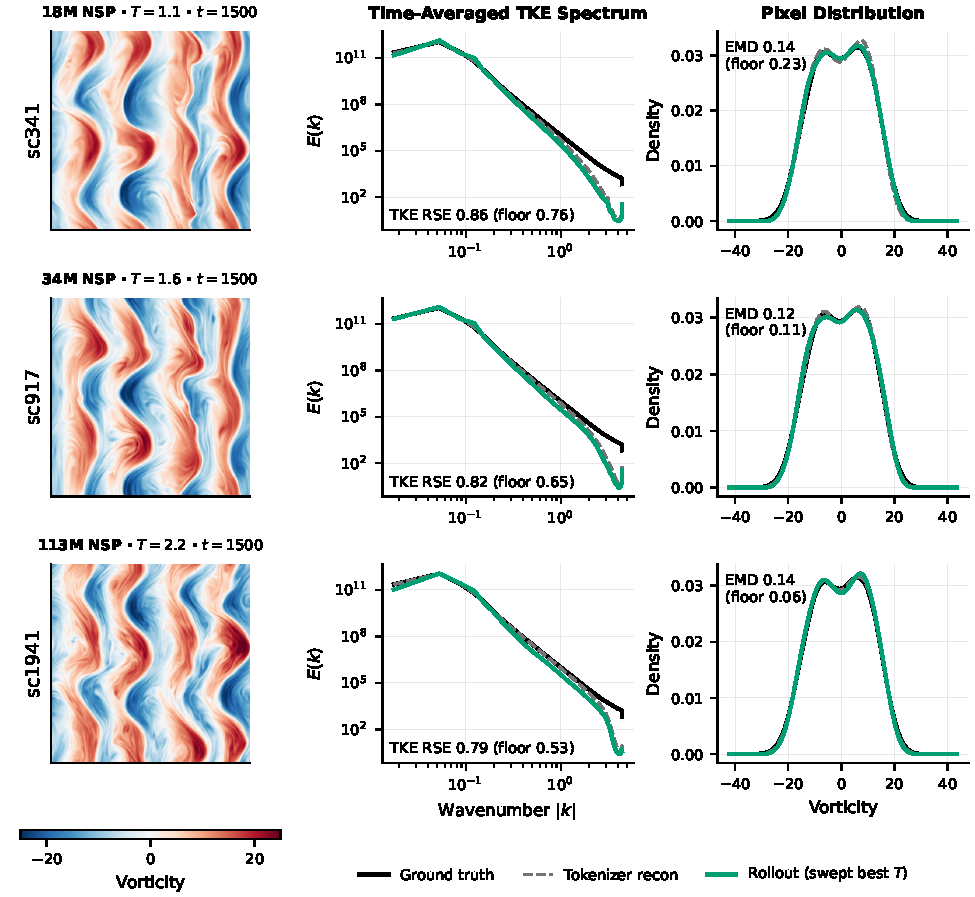
\includegraphics[width=\linewidth]{headline/perclass_rows}
\caption{The best cell of each tokenizer family at its swept-optimal temperature ($N{=}128$
rollouts of 2{,}000 steps, trajectory 0 shown). Left: the rollout field at $t{=}1500$.
Middle: the time-averaged TKE spectrum against ground truth and the tokenizer
reconstruction. Each rollout is on its own floor through the resolved range. Right: the
pixel distribution. Ensemble EMD against the floor is $0.14/0.23$ for sc341 (below floor
by mode-averaging), $0.12/0.11$ for sc917, and $0.14/0.06$ for sc1941.}
\label{fig:perclass}
\end{figure}

\subsection{Baselines}
\label{sec:baselines}

The continuous baseline behind Figure~\ref{fig:offmanifold} is the same ViT autoencoder
wired as a continuous next-frame regressor and rolled for 2{,}000 steps, in five arms:
plain, input-noise low and high, pushforward, and a medium-sized plain arm as a capacity
control. The plain arm's one-step spectrum is essentially exact (median $|\log_2|$
deviation 0.004), yet by the end of the rollout its mid-$k$ band sits at
$2.1$--$2.8{\times}$ reference, with low-$k$ inflating past step ${\sim}500$: one-step
metrics predict nothing about the closed-loop attractor.

The baseline pushforward wins across the time-averaged spectrum. It is
closer to ground truth than the tokenizer floor, the discrete ceiling, for
$k \gtrsim 0.5$ (Figure~\ref{fig:pushfwdexp}). 
If the quantity of interest is an ensemble-mean statistic, pushforward is the better tool
on this system: it beats the tokenizer floor across the spectrum and is 0.03 ahead of the
calibrated discrete arm on EMD. If the
quantity of interest is the statistic of any individual run, the comparison reverses. 

\begin{figure}[!htb]
\centering
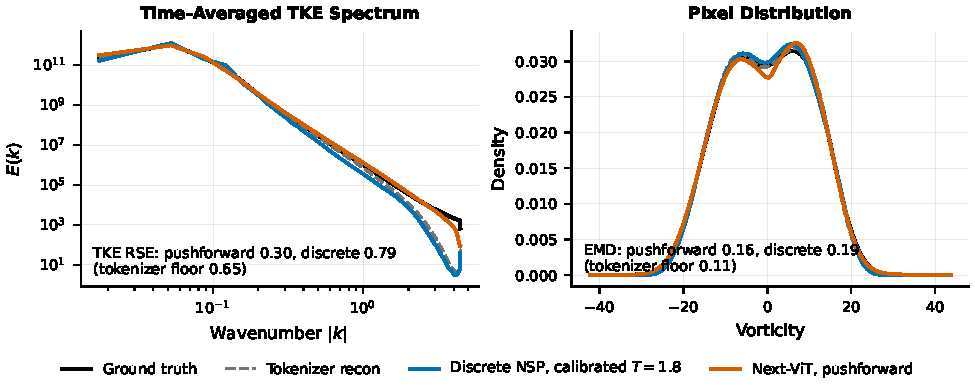
\includegraphics[width=\linewidth]{baselines/pushforward_expectation}
\caption{Every time-averaged metric prefers the pushforward baseline. Left: its time-averaged TKE
spectrum follows ground truth through the resolved range and beats the tokenizer floor,
the ceiling on any discrete arm (TKE RSE 0.30 against the floor's 0.65 and the calibrated
discrete rollout's 0.79). Right: its pixel distribution is closer to the data than the
calibrated discrete arm's by 0.03 on EMD (0.16 against 0.19). The calibrated discrete arm is
the medium-sc917-s34 cell of Table~\ref{tab:deploy} at its read rounded to the nearest swept
temperature ($T^\ast{=}1.873$, $T{=}1.8$), averaged over the 128 trajectories of the sweep
rollout; the pushforward arm is averaged over 16. Both panels are expectations over the
rollout. What a single run holds at any given step is the subject of
Figure~\ref{fig:concentration}, on the same rollouts (16 trajectories each, 2{,}000 steps).}
\label{fig:pushfwdexp}
\end{figure}

Figure~\ref{fig:concentration} puts each 2{,}000-step rollout against its own spectral
reference (the tokenizer reconstruction's long-run spectrum for the discrete arms, the
model's own one-step spectrum for the continuous ones), as median plus cross-trajectory
5--95\% band, per-step and 250-step-windowed. 
The calibrated discrete arm is the medium-sc917-s34 cell of Table~\ref{tab:deploy} at its
read rounded to the nearest swept temperature ($T^\ast{=}1.873$, $T{=}1.8$), and it
concentrates, meaning its windowed statistic settles into a narrow band as the window grows.
Its 250-step-windowed band, the cross-trajectory 5--95\% range of the windowed
energy ratio, has width 0.084 (bootstrap over trajectories, 5--95\%: 0.066--0.088). The
autocorrelation time of its per-step energy excursions, the lag at which a trajectory's
autocorrelation first falls below $1/e$, is 7--34 steps (median 10), and windowing shrinks
each trajectory's own per-step spread by a factor of 0.14--0.53 (median 0.36 over the 16
trajectories). We use the true system's own wander as the control.

\begin{figure}[!htb]
\centering
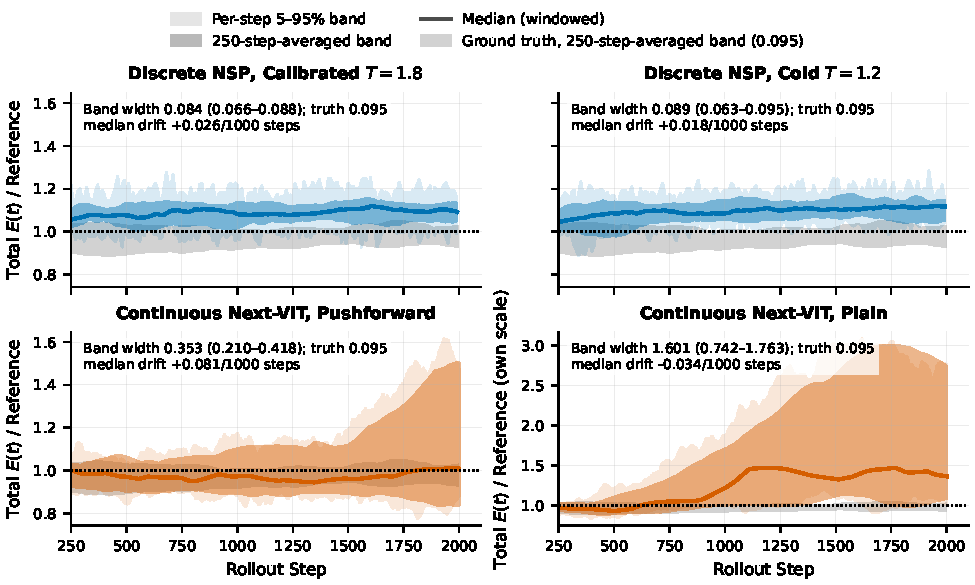
\includegraphics[width=\linewidth]{baselines/f71_stick_2x2_total}
\caption{Estimator concentration. Total spectral energy per step relative to each model's own
reference (the tokenizer reconstruction's long-run spectrum for the discrete arms, the
model's own one-step spectrum for the continuous ones), as the median and the cross-trajectory 5--95\% band, per-step (light) and
250-step-windowed (dark), with the 250-step spin-up cut. Gray is the ground truth's own
250-step-averaged band across fifteen disjoint 2{,}000-frame segments of the record,
width 0.095 (0.071--0.108). The discrete arms are the medium-sc917-s34 cell of
Table~\ref{tab:deploy}, 16 trajectories each, at its read rounded to the nearest swept
temperature ($T{=}1.8$) and at the cold edge of the sweep ($T{=}1.2$). The calibrated
discrete arm's windowed band is 0.084 (bootstrap over trajectories, 5--95\%: 0.066--0.088),
centered at 1.09. The cold discrete arm's band is 0.089 (0.063--0.095), and its collapse is
in the composition of the spectrum (Figure~\ref{fig:bandedconc}). The pushforward arm (16
trajectories) has a windowed band close to its per-step band, 0.353 (0.210--0.418). The
plain arm fans out to 1.60 (0.74--1.76).}
\label{fig:concentration}
\end{figure}

The control is the raw record cut into fifteen disjoint 2{,}000-frame segments treated as
trajectories and normalized by the held-out window's time mean. Its per-step band is 0.115
and its windowed band is 0.095 (bootstrap over segments, 5--95\%: 0.071--0.108), with
per-segment long-run means within 0.92--1.02 of the held-out reference (gray in
Figure~\ref{fig:concentration}). The calibrated
discrete arm's 0.084 lies inside the bootstrap interval of the true system's band,
0.071--0.108. The band is centered at 1.09 rather than at 1.0. 

Every trajectory's long-run total energy is 1.07--1.12 times its floor's, which is the low-$k$ excess of
Figure~\ref{fig:bandedconc}, so the arm concentrates on a total 9\% above its reference.
The cold discrete arm, the same cell at the cold edge of the sc917 sweep ($T{=}1.2$),
concentrates as well, with a windowed band of 0.089 (0.063--0.095), and its collapse is in
the composition of the spectrum rather than in the total. Its mid-$k$ band settles at
0.31--0.33 of the floor across trajectories against 0.57--0.61 at $T{=}1.8$, and its
high-$k$ band at 0.23--0.26 against 0.43--0.47. The high-$k$ band keeps draining until step
${\sim}1{,}100$, whereas the calibrated arm's bands are in place by step 50
(Figure~\ref{fig:bandedconc}). Colder still, the collapse reaches the total. The per-token
arm of the mask ablation (small-sc917-s34) at $T{=}0.7$ has a windowed band of 0.222
(0.144--0.235), and its low-$k$ band declines from 0.955 to 0.874 between the first and
last quarters of the run, which is the diffusive collapse as it appears in the spectra.

The continuous pushforward arm is stable in the ensemble mean only. Over 16 trajectories
its windowed band is 0.353 (0.210--0.418), close to its per-step band and 3.7 times the
true system's 0.095, under a coherent wander with an autocorrelation time of 37--195 steps
(median 82), with long-run mid-$k$ states spanning $0.91$--$1.69{\times}$ across the
trajectories, so no practical window captures what spectrum a single run holds. Within a trajectory, 
windowing shrinks the spread by 0.34--0.92 (median 0.65), so the per-trajectory ranges of the pushforward arm and
the calibrated discrete arm overlap, and the separation between them is in the
cross-trajectory band. An earlier run of this arm with eight
trajectories from a different set of initial conditions gave 0.232 (0.086--0.293), and adding
trajectories widened the band. We report the 16-trajectory value, and its bootstrap interval,
0.210--0.418, does not overlap the calibrated discrete arm's, 0.066--0.088.

The band a continuous arm settles into is set by its training procedure and
not by its architecture: the pushforward arm and the plain arm share an architecture, and
their windowed bands differ by a factor of ${\sim}4.5$ (0.353 against 1.60), so the
margin a system gets cannot be known before the rollout is run. The plain continuous arm accumulates error, with a windowed band of 1.60
(0.74--1.76) and growing while its one-step spectrum is exact. Against a common reference,
the ground-truth spectrum instead of each arm's own, the ordering holds. The windowed band
is 0.084 (0.066--0.088) for the calibrated discrete arm and 0.351 (0.209--0.416) for
pushforward. Every calibrated trajectory's long-run total energy lies within 1.07--1.12 of
the truth's, a narrow band 9\% high, against 0.85--1.28 for pushforward, a wide band
centered near the truth, and 1.07--1.14 for the cold discrete arm (Appendix~\ref{app:exhibits}, Figure~\ref{fig:concgt}).

The banded mechanism panels (Appendix~\ref{app:exhibits}, Figure~\ref{fig:bandedconc}) show the calibrated arm's deficit
relative to its own floor established within ${\sim}50$ steps and stationary thereafter
($|$slope$| \leq 0.02$ per 1000 steps over the second half in every band), with the total
9\% above the floor: the residual moves energy from mid and high $k$ to low $k$ rather than
losing it.


% =====================================================================
\section{Limitations}
\label{sec:limitations}

All results in this work come from one system: every claim is scoped to this 2D turbulence
dataset, and the demonstrated transfer is across 45 model/tokenizer configurations within
it rather than across PDEs. The global temperature read is a stability calibration and not an
accuracy optimizer. The read is warmer than the EMD-optimal swept temperature in nearly every
cell (Table~\ref{tab:outcome}), and a user who wants the lowest EMD on a cell still needs the
sweep. On sc341, where greedy decoding is already on-manifold in 14 of 15 cells, the
calibration prevents nothing and only adds regret, and its benefit is on the families with a
cold failure, sc917 and sc1941. A
calibration that is sweep-free and EMD-optimal at once remains open
(Appendix~\ref{app:future}). A
joint-level residual also remains: the calibrated rollout holds ${\sim}0.4$--$0.5{\times}$
of its own floor's band energy below the spectral peak. This residual is stationary,
energy-conserving, and countable, but it is real, and marginal calibration does not close
a joint statistic.

% =====================================================================
\section{Conclusion}
\label{sec:conclusion}

A discrete multi-scale surrogate holds the long-run statistics of 2D turbulence for
thousands of steps, and not because discreteness grants stability. Tokenization allows us
to determine instabilities by directly comparing live rollout statistics to the data
distribution, and stable rollouts require matching the two distributions. Marginal-entropy
calibration performs that matching with a few short diagnostic rollouts scored on their
own emitted tokens instead of a ground-truth-scored sweep; its target is computed from
the tokenizer and dataset alone, and ground truth enters only at evaluation, which makes
it a candidate default for the next system.
The calibration delivers a rollout that does not collapse and does not explode, and not
the lowest error. The calibrated temperature is warmer than the EMD-optimal swept
temperature in nearly every configuration, and the rollout at it scores a higher EMD than the
rollout at that optimum. That difference is the cost of not running the sweep. Open directions, including a per-scale
temperature, are in Appendix~\ref{app:future}.


\newpage

% From the references on, stop vertically justifying pages: the appendix's [H]
% figures force page breaks, and \flushbottom was stretching the glue between
% bib entries and appendix bullets into large mid-page gaps.
\raggedbottom
\bibliography{references}
\bibliographystyle{tmlr}

\newpage

\appendix

\section{Open directions}
\label{app:future}

Several directions remain open: the continuous-latent isolation, rolling out in latent
space without decoding at every step, the same calibration on PDEs we have not touched,
and a per-scale temperature (Figure~\ref{fig:perscalefuture}). The global read heats
every scale by the same amount, although the entropy drain it corrects is fastest at the
finest scales. On the sc1941 grid we ran
two per-scale schedules against the same $N{=}128$ sweep. A hand-set schedule that leaves
the coarse scales at $T{=}1$ and heats only the finest two, to one fixed value per VQ tier
chosen from the three we ran (3.0 under the small and medium VQ, 2.0 under the large), is
a median 0.01 EMD from the swept single-temperature optimum, against 0.11 for the global
read: below the optimum by more than 0.03 on 4 of 15 cells, within 0.03 on 6, and above it
on 5, one of those above the explosion bar (small VQ, 31M NSP, EMD 1.16 where the global
read's rollout has EMD 0.79). Its spectral error is below the optimum's on 11 of 15. The solved schedule,
one temperature per scale matching that scale's emitted entropy to the training set's,
ends up close to the global read: on the coarse scales and on the finest scale the rollout's emitted
entropy never reaches the training set's at any temperature we swept, so 51 of the 90
scale-temperatures pin to the hottest swept temperature, 2.2, the finest scale on every
cell, and the result is a near-flat schedule whose EMD is below the global read's on 10 of 15
cells (median 0.26 against 0.31) and below the swept optimum on none. The solved schedule
also concentrates the way the global read does. On the same 15 cells the 250-step-windowed
band of Section~\ref{sec:baselines} is 0.067--0.119 (median 0.080) for the solved schedule
and 0.058--0.091 (median 0.076) for the global read, within 0.034 of each other on every
cell, and the band's center is between 0.94 and 1.03 of the tokenizer floor for both.
Concentration is a property of the discrete rollout at any sampled temperature, including
the medium-VQ 139M cell's read at $T{=}2.6$ with EMD 0.80, and not of the schedule. The
schedules differ in the level at which the mid-$k$ band settles and not in the band's width.
Heating the coarse
scales alone to 2.0 explodes the same four cells greedy does. Solving for the fine-scale
temperatures from the training-set entropy, instead of choosing them by hand, is the open
step.

\begin{figure}[H]
\centering
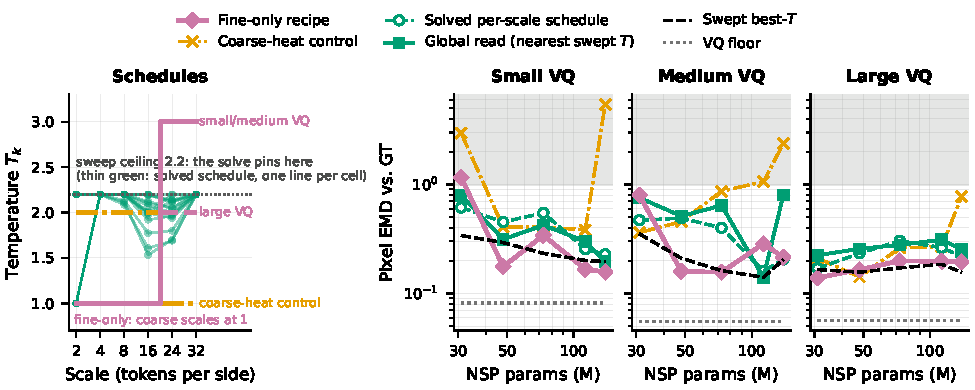
\includegraphics[width=\linewidth]{per_scale_temp/perscale_future_work}
\caption{Per-scale temperature as an open direction, on the sc1941 grid. Left: temperature per
scale for three schedules. The solved per-scale schedule (thin green, one line per cell)
matches each scale's emitted entropy to the training data's. On the coarse scales and the
finest scale the emitted entropy never reaches the data's at any swept temperature, so the
solve pins to the hottest swept temperature of 2.2 (dotted) on 51 of 90
scale-temperatures, and scale 2 falls back to $T{=}1$ where its response is flat. The
hand-set fine-only recipe (purple) leaves the coarse scales at 1 and heats the finest two
to 3.0 under the small and medium VQ and 2.0 under the large, and the coarse-heat control
(gold) is its mirror. Right: pixel EMD of those arms against NSP size per VQ tier, with
the global read (green squares) and the swept best-$T$ yardstick (dashed). Every sampled
arm is $N{=}128$ trajectories of 2{,}000 steps, and the gray band is EMD above the
explosion bar. The fine-only recipe is on the yardstick where the global read is above it and
explodes on one cell, and the coarse-heat control explodes on the four cells greedy
does.}
\label{fig:perscalefuture}
\end{figure}


% =====================================================================
% Appendix reordered 08-04 (user): leading exhibits first (fig:hierarchy,
% fig:temprows, fig:bandedconc, fig:singlestep, fig:modea in that order), then
% tokenizer analysis (the old Appendix B), then the support-mask ablation, then
% the remaining secondary results. Captions are self-contained; the argument
% prose stays in its home section and cross-references these figures.
\section{Extended exhibits}
\label{app:exhibits}

\begin{figure}[H]
\centering
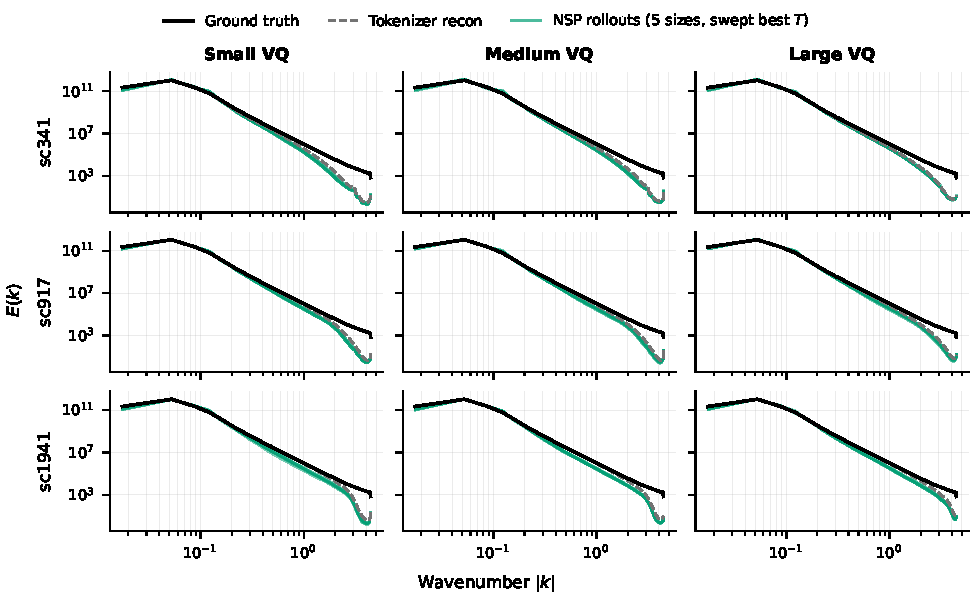
\includegraphics[width=\linewidth]{grids/analysis_tke_spectrum}\\[4pt]
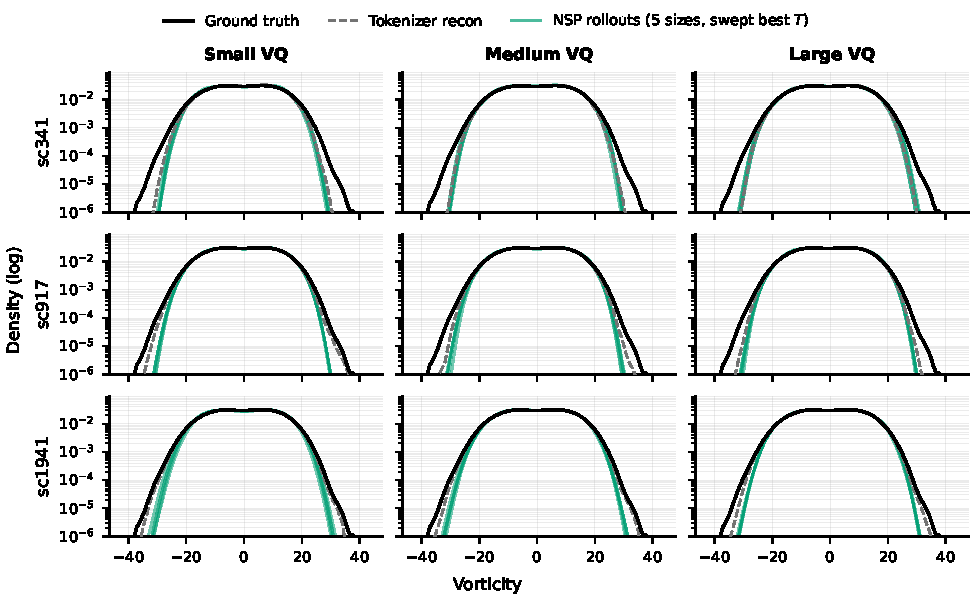
\includegraphics[width=\linewidth]{grids/analysis_pixel_histogram}
\caption{Time-averaged TKE spectra (top) and pixel PDFs (bottom) for every cell of the 45-cell
grid, the full grid behind the per-family exhibit of
Figure~\ref{fig:perclass}.}
\label{fig:hierarchy}
\end{figure}

\begin{figure}[H]
\centering
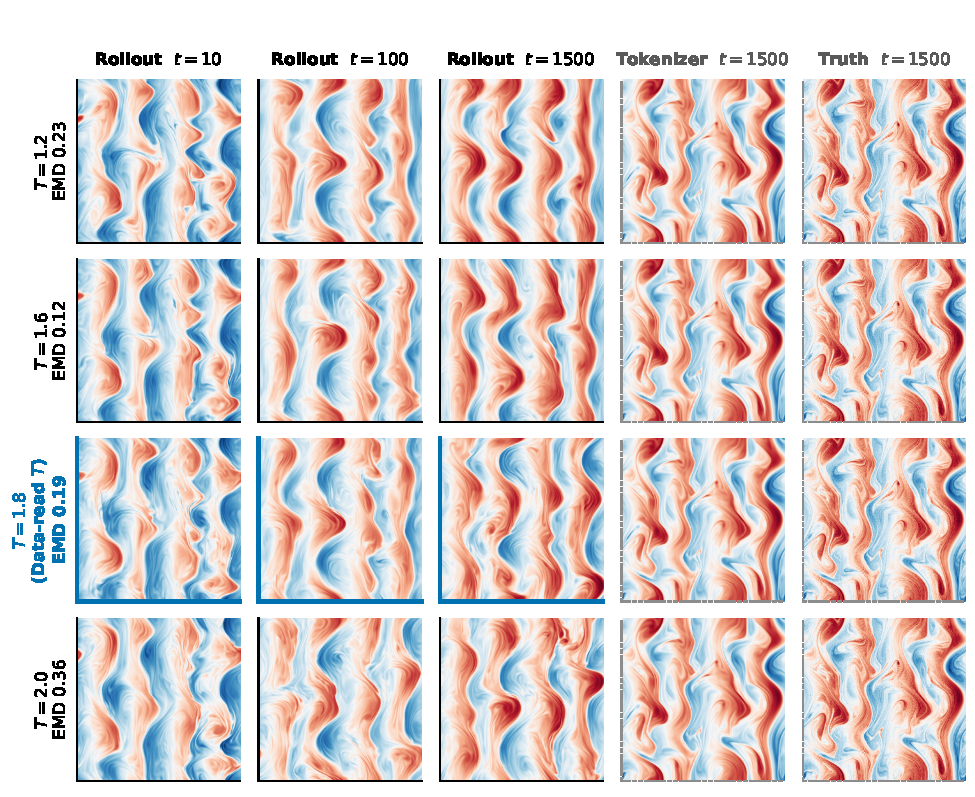
\includegraphics[width=\linewidth]{snapshots_n128_tempcollapse/medium-sc917-nsp-s34_temp_rows}
\caption{One row per sampling temperature for medium-sc917 (trajectory 0). Each row shows the
rollout at $t{=}10/100/1500$ with the tokenizer reconstruction and the ground truth at
$t{=}1500$. Cold sampling ($T{=}1.2$) fades toward smooth banding, the swept optimum $T{=}1.6$ and
the read ($T^\ast{=}1.873$, rounded to the swept $T{=}1.8$ and framed) keep the texture of
the references, and $T{=}2.0$ roughens. The
per-row ensemble EMD ($N{=}128$) is at left.}
\label{fig:temprows}
\end{figure}

\begin{figure}[H]
\centering
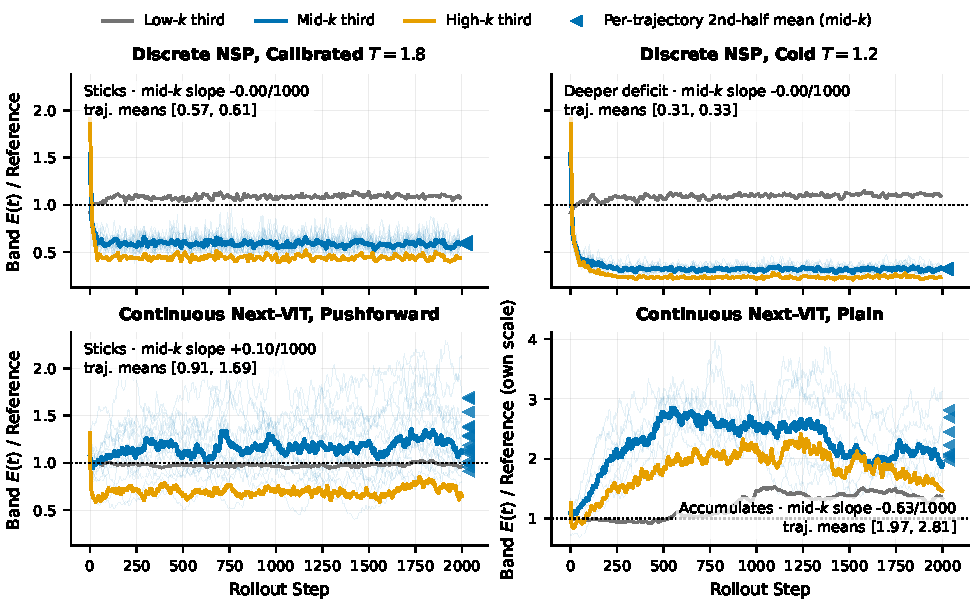
\includegraphics[width=\linewidth]{baselines/f71_stick_2x2}
\caption{Banded concentration panels, the mechanism behind Figure~\ref{fig:concentration}.
Per-step band-energy ratios against each arm's own reference (the tokenizer
reconstruction's spectrum for the discrete arms, the model's one-step spectrum for the
continuous ones) in the low, mid, and high $k$-thirds, with the median line and per-trajectory end-of-run ticks.
The calibrated discrete arm holds its mid-$k$ band at 0.57--0.61 of its floor across
trajectories and the cold arm at 0.31--0.33; the pushforward arm's trajectories span
0.91--1.69.}
\label{fig:bandedconc}
\end{figure}

\begin{figure}[H]
\centering
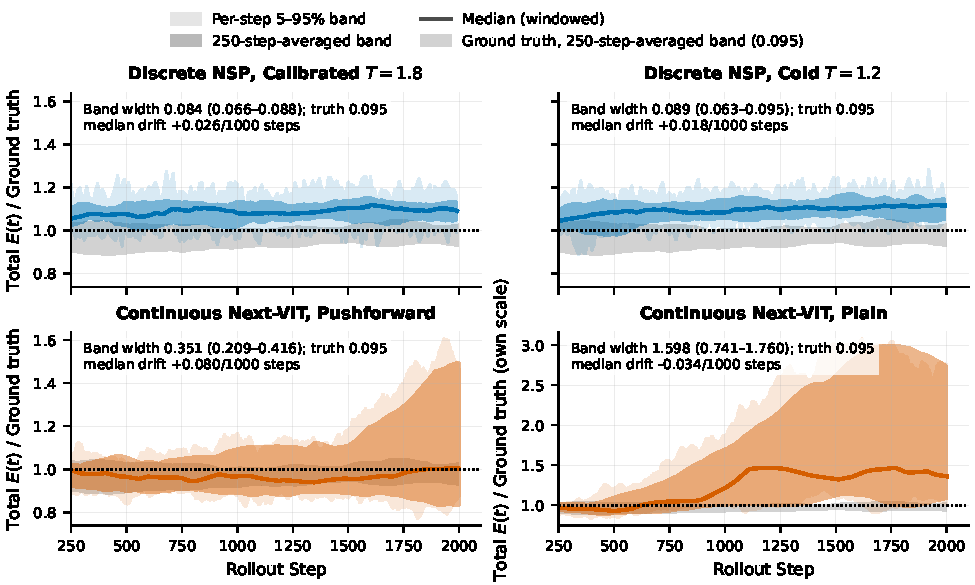
\includegraphics[width=\linewidth]{baselines/f71_stick_2x2_total_vs_gt}
\caption{Figure~\ref{fig:concentration} against a common reference. Total spectral energy per
step relative to the ground-truth spectrum for every arm, as the median and the
cross-trajectory 5--95\% band, per-step (light) and 250-step-windowed (dark), with the
windowed band width and its bootstrap interval over trajectories.}
\label{fig:concgt}
\end{figure}

\begin{figure}[H]
\centering
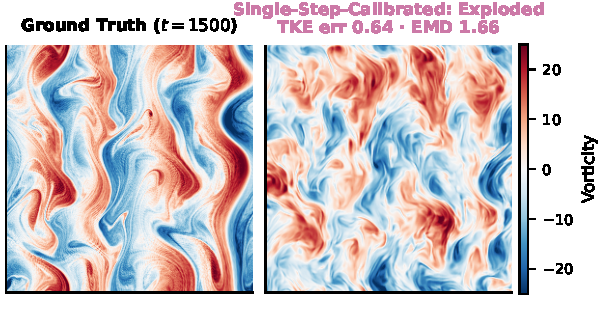
\includegraphics[width=0.62\linewidth]{inference_samplers/singlestep_exploded}
\caption{What the single-step route produces in rollout. Ground truth at $t{=}1500$ (left) next to
a single-step-calibrated rollout at the same lead time (right), with the entropy targeted
to the per-position tokenizer marginal on small-sc1941. Its EMD is 1.66, and the spectrum
forgives it again with a TKE error of 0.64 against 0.88 for the greedy-collapsed arm of
Figure~\ref{fig:failuremodes}. Every
single-step-driven arm leaves the manifold on every configuration that needs warmth.}
\label{fig:singlestep}
\end{figure}

\begin{figure}[H]
\centering
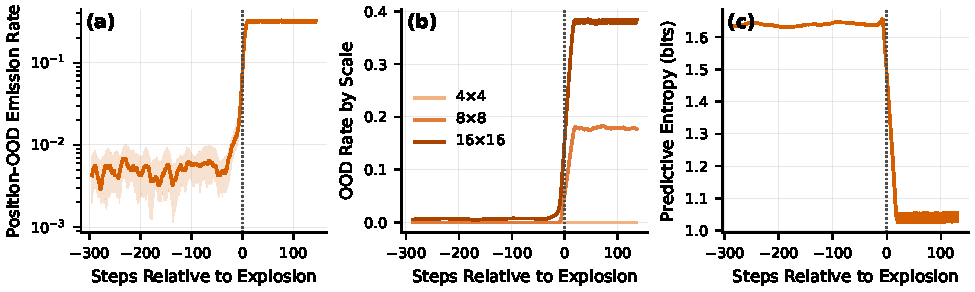
\includegraphics[width=\linewidth]{mode_diagnostics/mode_a_aligned}
\caption{The explosion failure, diagnosed from the model's own emissions. 21 of 25 unconstrained
sc341 trajectories (per-scale-mask era, $T{=}1.0$) explode, and the traces are aligned at
each trajectory's OOD avalanche (median, IQR shaded). Left: the per-position OOD emission
rate. Middle: the avalanche by scale; the coarse scales never leak. Right: predictive
entropy, flat until the explosion and then confident static.}
\label{fig:modea}
\end{figure}

% =====================================================================
\section{Tokenizer analysis}
\label{app:tokenizer}

We evaluated flat and multi-scale tokenizers at fixed autoencoder size through one evaluation path. Multi-scale has no reconstruction advantage at matched
token budget (Table~\ref{tab:reconfloor}). Scale count moves the floor and autoencoder
size does not, with utilization at ${\sim}59\%$ and zero dead codes, so the floor is a
scale-resolution and deterministic-argmax bound rather than a capacity bound
(Figure~\ref{fig:vqsizefloor}).

\begin{table}[H]
\centering
\caption{Validation-window reconstruction floors for flat and multi-scale tokenizers at the fixed
Small autoencoder size.}
\label{tab:reconfloor}
\begin{tabular}{lrrrrr}
\toprule
tokenizer & tokens/frame & EMD & TKE RSE & mid-$k$ ret. & codes used \\
\midrule
flat-256    & 256   & 0.217 & 0.776 & 0.128 & 1095 \\
sc341       & 341   & 0.400 & 0.799 & 0.106 & 741  \\
flat-576    & 576   & 0.142 & 0.687 & 0.296 & 1171 \\
flat-1024   & 1024  & 0.108 & 0.619 & 0.437 & 275  \\
sc917       & 917   & 0.107 & 0.644 & 0.395 & 2517 \\
sc1941      & 1941  & 0.085 & 0.546 & 0.595 & 2110 \\
\bottomrule
\end{tabular}
\end{table}

\begin{figure}[H]
\centering
\begin{subfigure}{0.44\linewidth}
  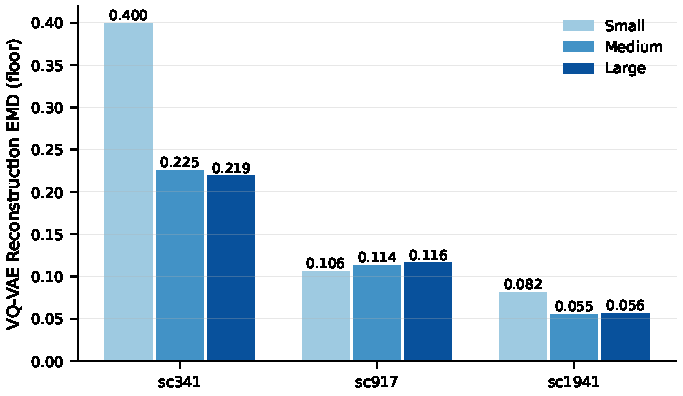
\includegraphics[width=0.7\linewidth]{recon_floor/vq_size_floor}
  \caption{VQ size vs floor}
\end{subfigure}
\hfill
\begin{subfigure}{0.52\linewidth}
  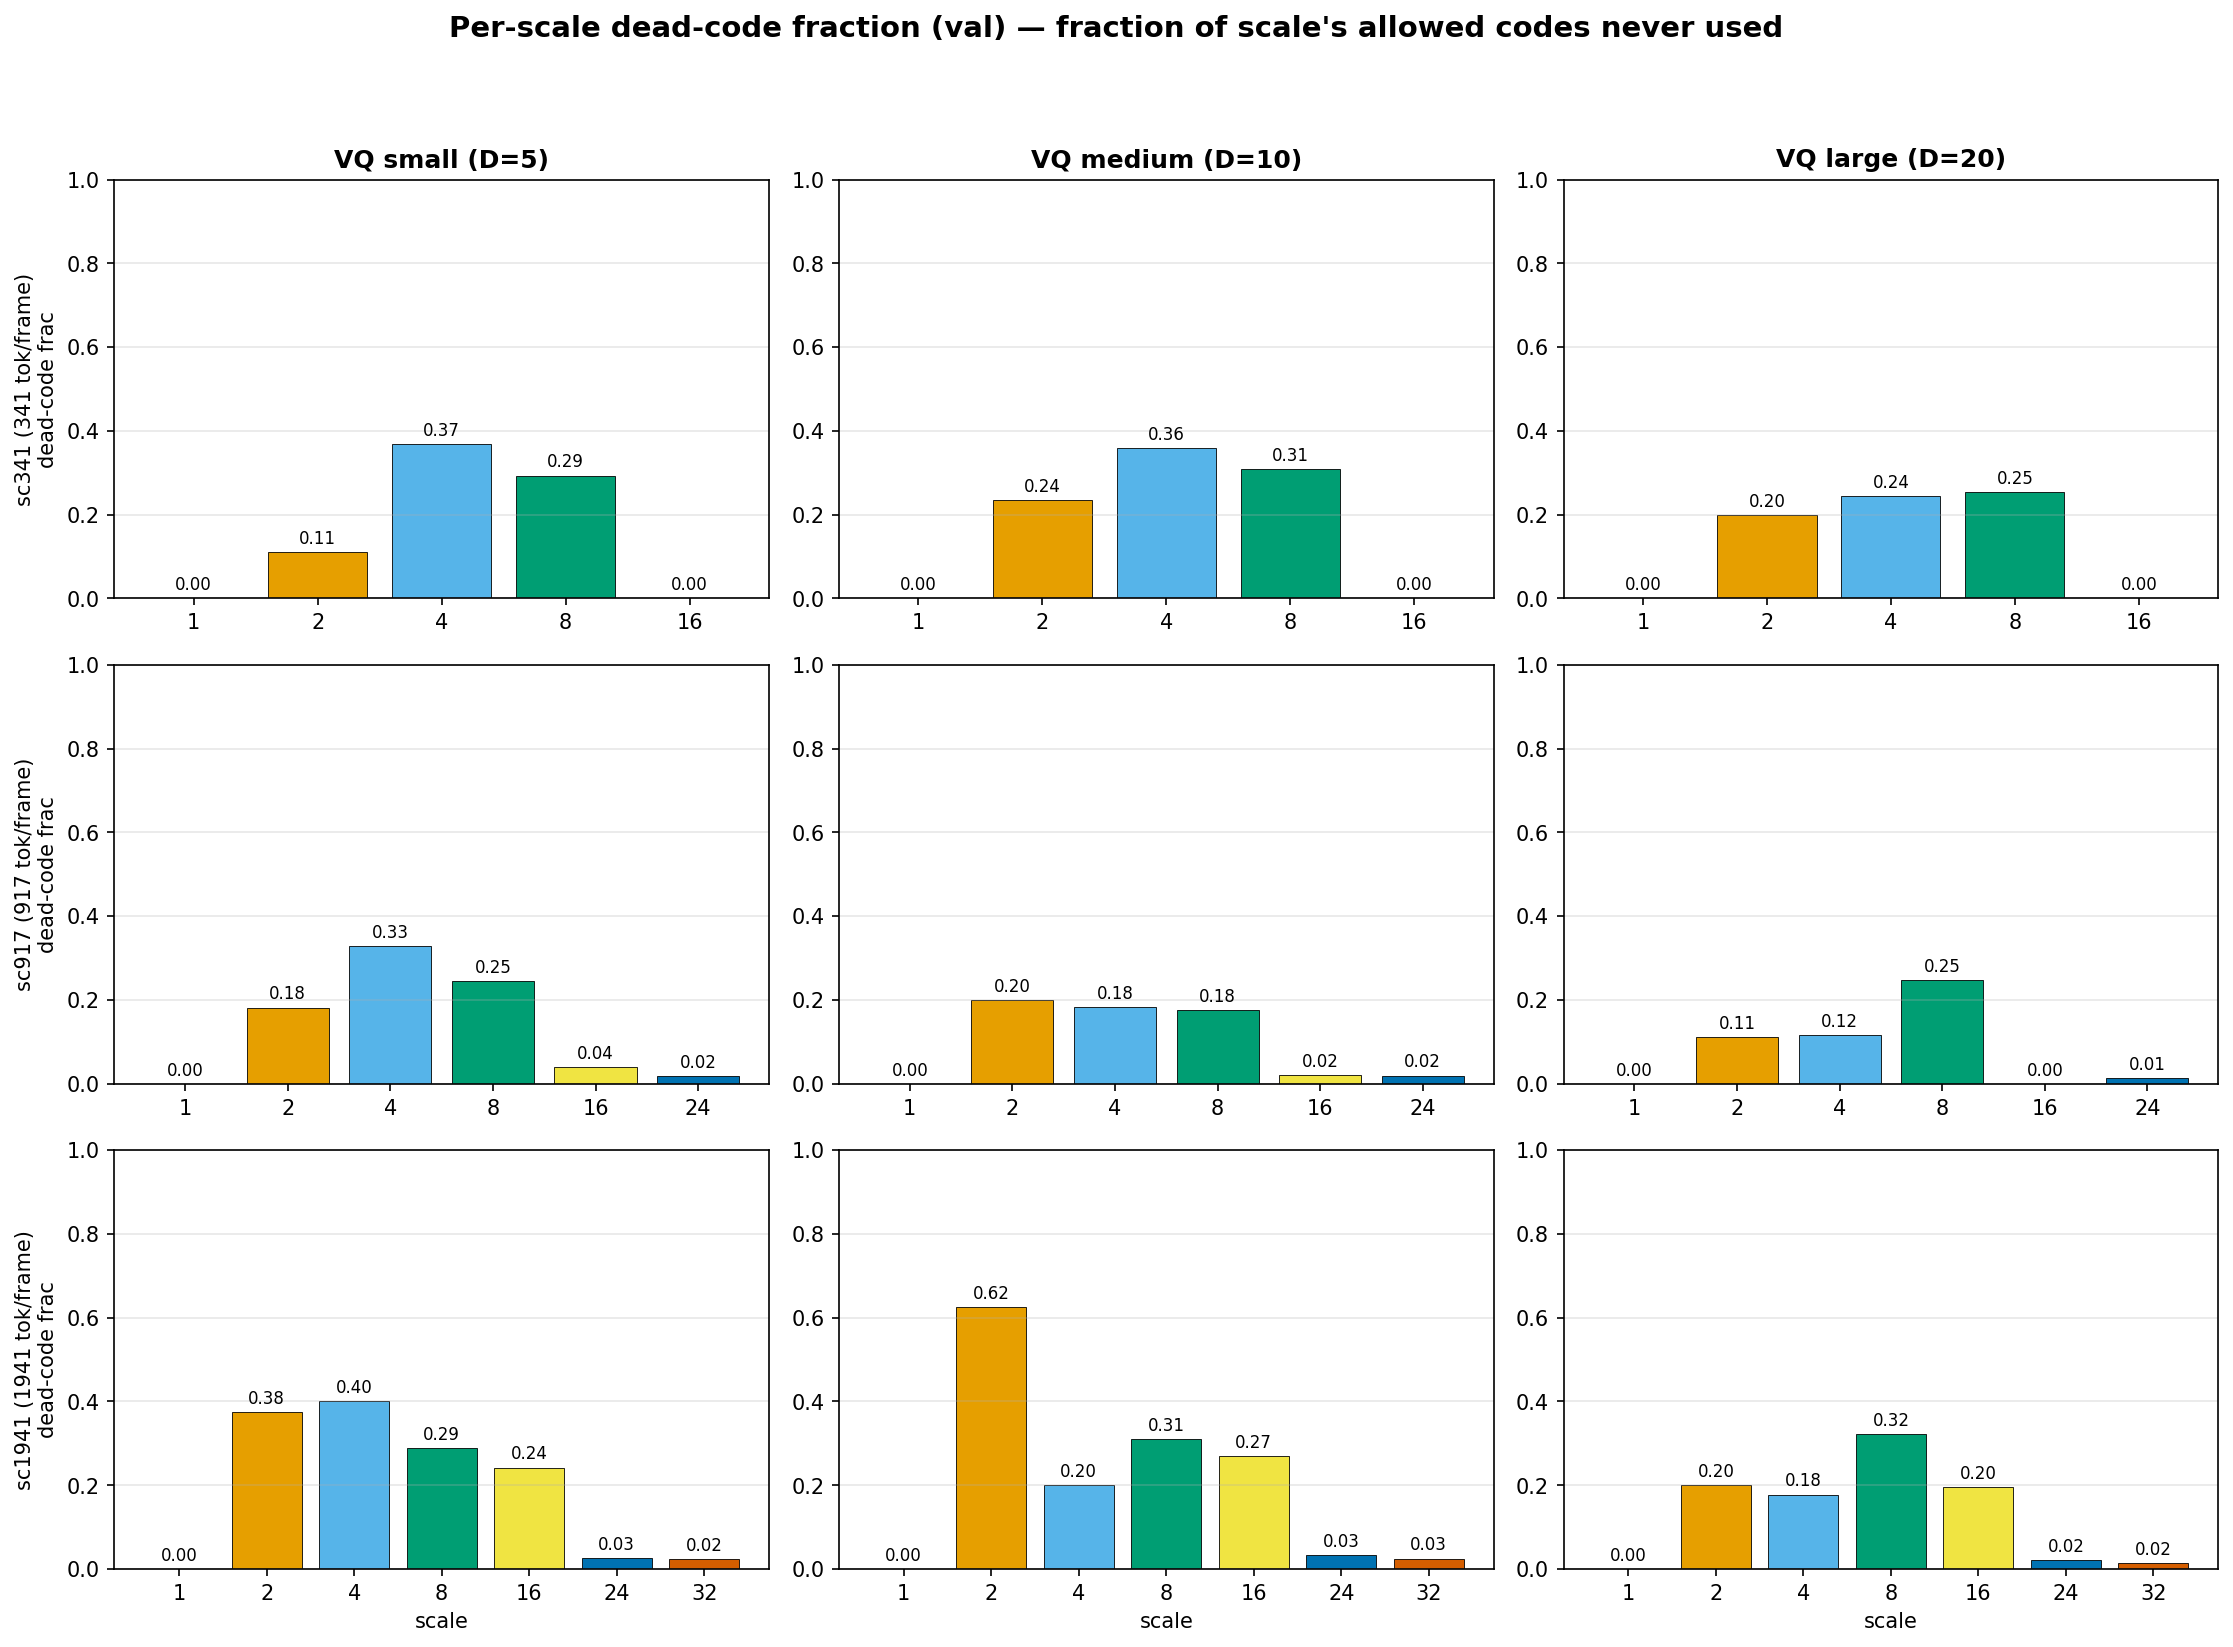
\includegraphics[width=\linewidth]{codebook_analysis/utilization_dead_codes}
  \caption{codebook utilization}
\end{subfigure}
\caption{(a) Scale count moves the floor and autoencoder size does not. (b) Codebook utilization,
with zero dead codes.}
\label{fig:vqsizefloor}
\end{figure}

% =====================================================================
\section{Choice of support mask}
\label{app:mask}

% Why per-position is the default: a story about both failure directions. The line the
% appendix argues: a bad mask does not give a stable rollout; it gives a choice of failure.

Without a position-level constraint, sampling occasionally emits a token never seen at
that position. The decoder maps it to high-frequency static, the next step conditions on
the static, and the rollout explodes within tens of steps. In 21 of 25 unconstrained sc341
trajectories the rollout ends this way (Figure~\ref{fig:modea}), with a stationary
position-OOD rate of 0.5\% avalanching to 30\% locked to the explosion and the violations
concentrated at the fine scales. No mask of any granularity prevents the diffusive
collapse, since every cold arm degrades whatever the constraint (EMD 0.42--0.65;
Table~\ref{tab:maskablation}). The two failures have opposite token-space signatures,
off-support and loud against in-support and quiet, which is why they cannot share a
detector.

The per-position mask makes the explosion structurally impossible: survival on the
pre-era cell goes from 0--4\% to 100\% (Figure~\ref{fig:survival}), and the OOD counter
becomes an exact alarm. On credit assignment (Figure~\ref{fig:maskablation}), a
noise-trained model respects scale-level support on its own ($1.5{\times}10^{-6}$
violations per token) but not position-level support (a stationary $3.5{\times}10^{-3}$,
touching 96\% of frames). A per-scale mask leaves that rate unchanged, and only the
per-token mask closes it, exactly.

\begin{figure}[H]
\centering
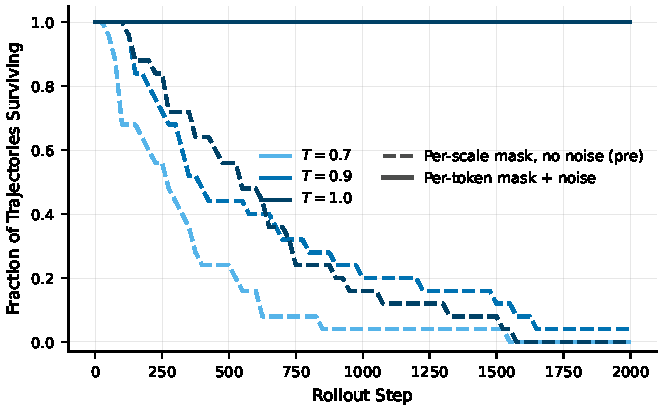
\includegraphics[width=0.68\linewidth]{mode_diagnostics/survival_beforeafter}
\caption{Survival before and after the per-position mask and substitution noise on the same sc341
cell, 25 trajectories per arm. Every pre-era arm dies (0--4\% by step 2000) and every masked arm survives to the
horizon. The pre-era arms also lack substitution noise, so mask and noise are jointly
credited here, and the ablation of Figure~\ref{fig:maskablation} separates them. The
survival bar, an EMD of twice the tokenizer floor, over-flags low-floor tokenizers and is
used only here.}
\label{fig:survival}
\end{figure}

\begin{figure}[H]
\centering
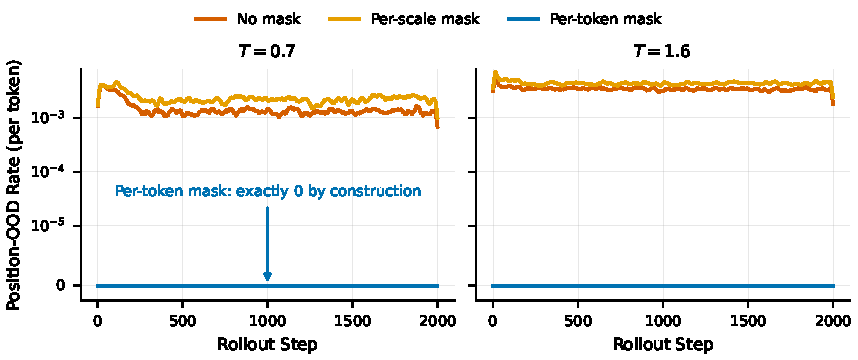
\includegraphics[width=0.88\linewidth]{mask_ablation_ood/ood_rate_traces}\\[6pt]
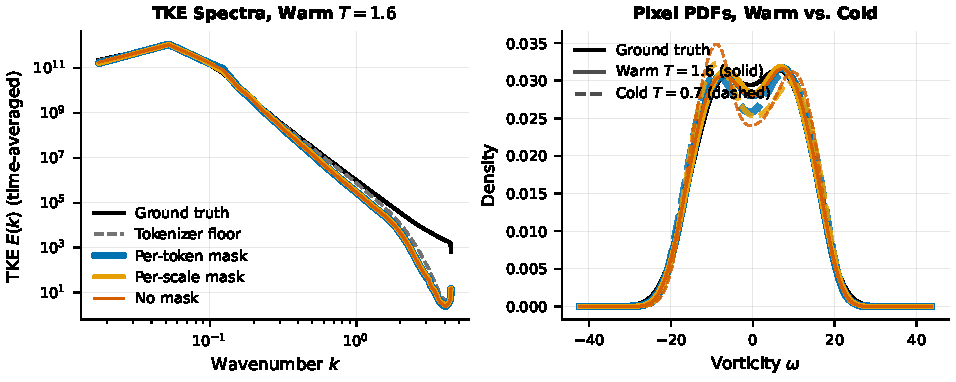
\includegraphics[width=0.98\linewidth]{mask_ablation_ood/mask_ablation_spectra}
\caption{Mask-granularity ablation. Three arms on one sc917 cell with identical training,
including 0.10 substitution noise, rolled out cold and warm. Top: position-OOD emission.
The per-scale mask overlays no-mask, and per-token is exactly zero. Bottom left: the warm
spectra coincide. Bottom right: pixel PDFs; the cold arms (dashed) over-sharpen regardless
of mask. Temperature separates the outcomes, and the mask contributes the guarantee and
the alarm.}
\label{fig:maskablation}
\end{figure}

\begin{table}[H]
\centering
\caption{Rollout EMD per arm of the mask ablation (tokenizer floor 0.106). The warm arms are all
healthy while their OOD behavior differs by three orders of magnitude, and cold sampling
collapses all three.}
\label{tab:maskablation}
\begin{tabular}{lccc}
\toprule
 & no mask & per-scale & per-token \\
\midrule
warm $T{=}1.6$, EMD          & 0.212 & 0.165 & 0.182 \\
cold $T{=}0.7$, EMD          & 0.645 & 0.566 & 0.421 \\
warm pos-OOD rate (/token)   & $3.5{\times}10^{-3}$ & $4.4{\times}10^{-3}$ & 0 \\
\bottomrule
\end{tabular}
\end{table}

% =====================================================================
\section{Secondary results and deferred comparisons}
\label{app:secondary}

As controls on the calibration, we tried anchoring the emitted-token entropy to the
model's own predictive entropy instead of the training-set entropy. This solves to
$T_k \approx 1$ identically, since a sampler that restores the model's own entropy cannot
warm by construction. The cross-entropy anchor of Section~\ref{sec:gate}, which matches
the softmax entropy to the teacher-forced cross-entropy per scale, is the strongest
teacher-forced variant, and it fails for the reason measured there. The
seven single-step-adaptive samplers give the same negative in its broadest form. The arms
are three entropy-targeting homeostats in the style of Mirostat \citep{basu2021mirostat},
aimed at the pooled marginal, the per-position marginal, and the model's own predictive
entropy, top-H \citep{baghaeipotraghloo2025toph}, typical sampling
\citep{meister2023typical}, min-p \citep{nguyen2025minp}, and an entropy-dependent
temperature with inverted polarity \citep{zhang2024edt}. At scales whose conditional
entropy is near zero there is nothing for an adaptive gate to fire on
(an exemplar field is in Figure~\ref{fig:singlestep}).
% PROSE NOTE (07-21, installed 08-25): this is the reader's ONLY meeting with these
% samplers. Arm -> cite map (verified against samplers.py): etpool/etpos/etmodel ->
% basu2021mirostat (entropy-target homeostat), tophabs -> baghaeipotraghloo2025toph,
% typical -> meister2023typical, minp -> nguyen2025minp, invedt -> zhang2024edt
% (inverted polarity); top-k/top-p ancestral -> fan2018hierarchical/holtzman2020degeneration.

Figures~\ref{fig:global917} and~\ref{fig:global341} are the sc917 and sc341 analogs of
the Figure~\ref{fig:schedule} grid, built the same way from the global-temperature sweep.
sc917 behaves like sc1941. Greedy decoding is above the swept optimum, the swept
temperature with the lowest ensemble EMD on the cell, by 0.04 to 1.71 EMD on 14 of its 15
cells and explodes on 2, the cold sweep edge ($T{=}1.2$) is above the swept optimum by a
median 0.17 EMD (0.05 to 0.53), and the calibrated read rounded to the nearest swept
temperature is within 0.08 EMD of the swept optimum on 10 cells and above it by 0.15 to
0.57 on the other 5. sc341 is the mirror image
and is stable cold. Greedy decoding is within 0.08 EMD of the swept optimum on 14 of its
15 cells, below it on 5 of them, and dips below the tokenizer floor by mode-averaging,
while the calibrated read is warmer than the swept optimum
and stays on-manifold. The EMD regret of the read is largest on this family: median 0.26
against 0.14 on sc917 and 0.13 on sc1941 (Figure~\ref{fig:regret}).

A stochastic sampler gives ensembles from a fixed initial condition for free, where
deterministic surrogates need IC perturbation and inherit its arbitrariness. Concentration
(Section~\ref{sec:baselines}) makes such an ensemble interpretable: a single rollout's
windowed estimate of the long-run statistics converges at a known rate
(an autocorrelation time of 7--34 steps), so the spread across seeds measures sampling
uncertainty rather than slow wander. The figures behind the metric protocol of
Section~\ref{sec:metrics} are the per-temperature snapshot rows (Figure~\ref{fig:temprows})
and the (cell,\,$T$) phase diagram whose stars are the calibrated reads
(Figure~\ref{fig:phasediagram}). The banded concentration panels
(Figure~\ref{fig:bandedconc}), the mechanism behind Figure~\ref{fig:concentration}, show
the low-$k$ band-energy ratio held between 1.04 and 1.14 for 2{,}000 steps at the
calibrated $T$, the mid and high bands settling within ${\sim}50$ steps and stationary
thereafter, and per-trajectory long-run mid-$k$ states spanning 0.57--0.61 for the
calibrated discrete arm against 0.91--1.69 for pushforward. The forecast-optimal temperature is cold, at the cold edge of the swept
bracket and so only a lower bound, while the long-run optimum is warm.
% SPLIT RESOLVED (user, 08-03): rerun on a pure validation window, no changes;
% forecast evals included.
Twelve sc341 cells roll out below their own tokenizer floor by mode-averaging, and sc917
and sc1941 never do.

\begin{figure}[H]
\centering
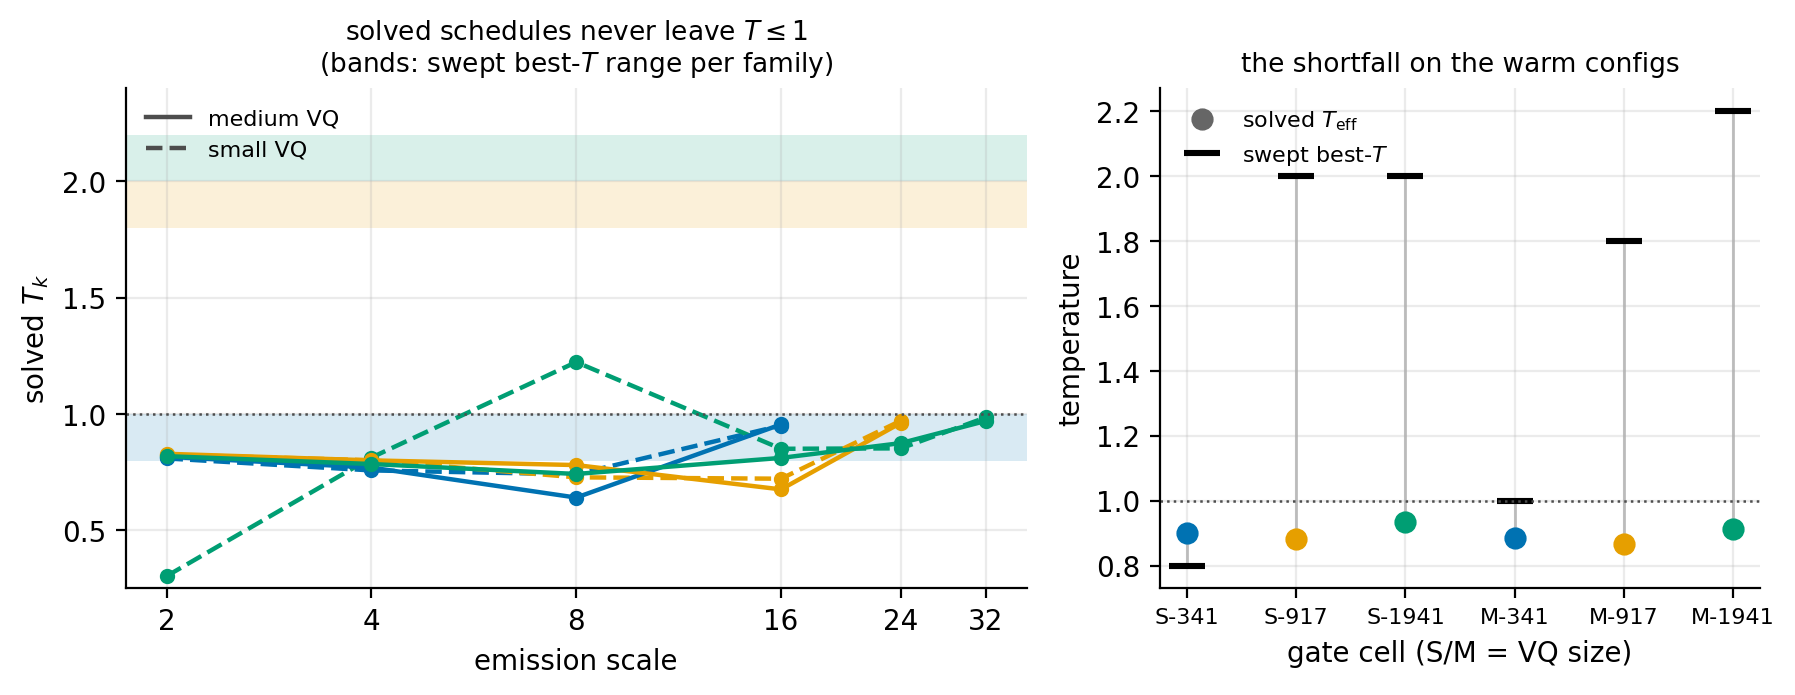
\includegraphics[width=0.95\linewidth]{calibration_gate/calib_gate_negative}
\caption{The strongest single-step anchor (CE matching), measured. Left: the solved per-scale
temperatures stay at $T\leq 1$, against the shaded bands of the swept best-$T$ ranges.
Right: the solved $T_{\text{eff}}$ against the swept best-$T$ per cell. sc341 passes, and
the warm configurations miss by a full temperature unit.}
\label{fig:calibgate}
\end{figure}

\begin{figure}[H]
\centering
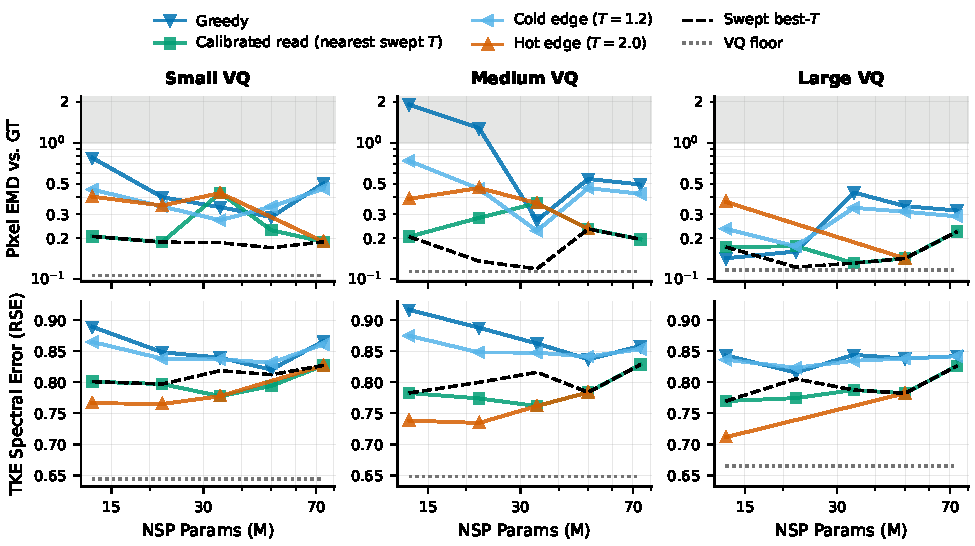
\includegraphics[width=\linewidth]{per_scale_temp/global_outcome_sc917}
\caption{The sc917 analog of Figure~\ref{fig:schedule}, from the global-temperature sweep (greedy
$N{=}1$, sampled arms $N{=}128$). Greedy and the cold sweep edge are above the swept
best-$T$ yardstick on EMD and have the largest TKE spectral error, and the calibrated global
read (rounded to the nearest swept temperature) is on the yardstick on 10 of the 15 cells.
This figure shows the original sweep range, whose hot edge on this family is $T{=}2.0$, so
the over-heat failure is not resolved here. The hotter points added to six sc917 cells are
in Figure~\ref{fig:phasediagram}.}
\label{fig:global917}
\end{figure}

\begin{figure}[H]
\centering
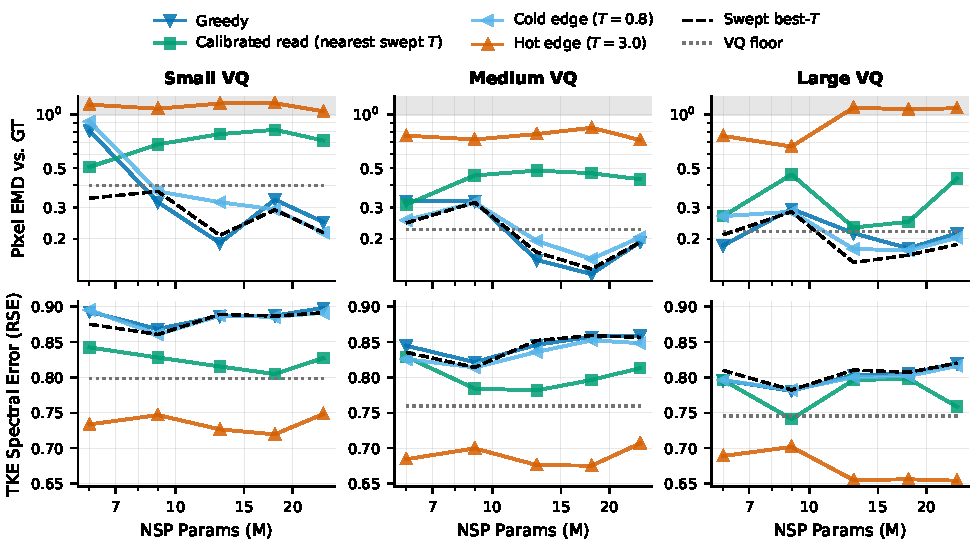
\includegraphics[width=\linewidth]{per_scale_temp/global_outcome_sc341}
\caption{The sc341 analog of Figure~\ref{fig:schedule}. This family is stable cold. Greedy and the
cold edge are within 0.12 EMD of the swept optimum on 14 of the 15 cells and dip below the
tokenizer floor by mode-averaging, while the calibrated read
is warmer than the swept optimum and stays on-manifold, so the read's regret, its EMD
above the swept optimum's, is largest on this family. The hot edge ($T{=}3.0$) shows the spectral camouflage at its
starkest, with EMD at the explosion bar and the lowest TKE error of any arm.}
\label{fig:global341}
\end{figure}

\begin{figure}[H]
\centering
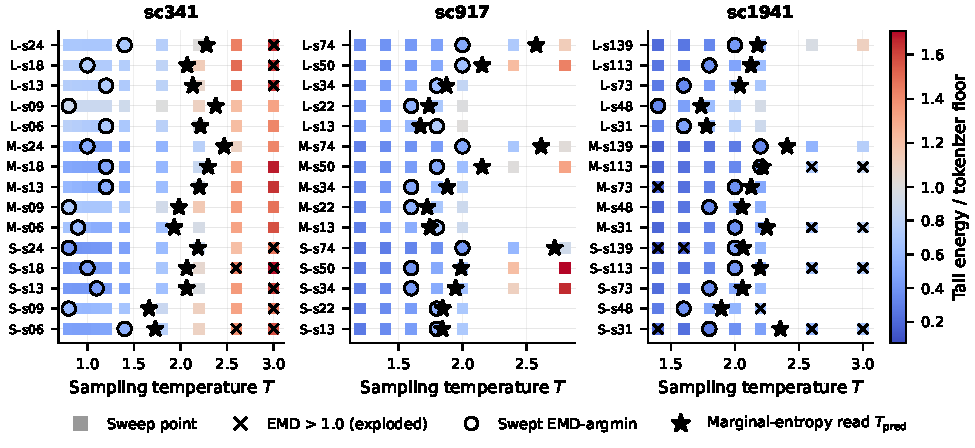
\includegraphics[width=\linewidth]{phase_diagram/phase_diagram_v1}
\caption{Temperature phase diagram. Every (cell, $T$) point of the $N{=}128$ sweep, colored by the
decoded tail energy relative to the tokenizer floor (the wavenumbers beyond the resolved
range); points whose ensemble EMD exceeds the explosion bar of 1.0 are crossed out. Per
cell, the open circle is the swept EMD-argmin and the star is the calibrated read.
The read lies inside the non-exploded interval in 42 of the 45 cells and between the
hottest non-exploded and the first exploded swept temperature in the other three, and is
warmer than the argmin in 43 of the 45. The finest-two-scale entropy gap $\Delta H$ has
rank correlation 0.87 with the tail energy relative to the floor across the 326 points,
and the star is its zero crossing.}
\label{fig:phasediagram}
\end{figure}

\begin{figure}[H]
\centering
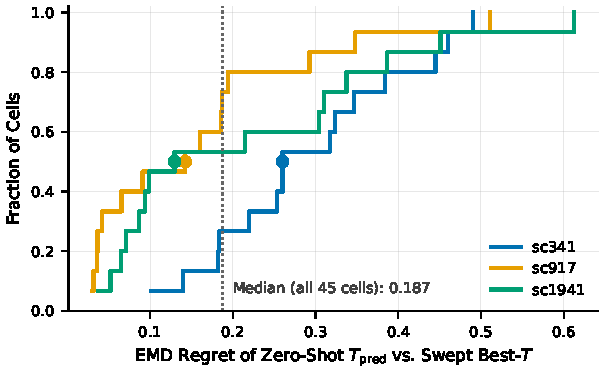
\includegraphics[width=0.62\linewidth]{regret/regret_distribution}
\caption{The EMD regret of the read. Per-family ECDFs of regret, the ensemble EMD at the read
minus the ensemble EMD at the cell's swept optimum. The median is 0.19 over all 45 cells: 0.26 on sc341, where the read is warmer
than the EMD-argmin in every cell while the rollout stays on-manifold, 0.14 on sc917, and
0.13 on sc1941.}
\label{fig:regret}
\end{figure}

\begin{figure}[H]
\centering
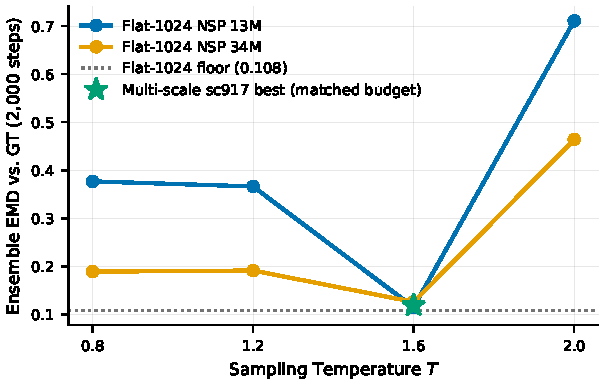
\includegraphics[width=0.62\linewidth]{baselines/flat_nsp_verdict}
\caption{The flat-NSP dynamics verdict. Ensemble EMD over 2{,}000-step rollouts against sampling
temperature for two NSP sizes trained on flat-1024 tokens, with the flat-1024
reconstruction floor. Flat holds the horizon at a swept $T{=}1.6$, essentially at floor and
level with the matched-budget multi-scale best (star: medium-sc917 at its swept optimum,
EMD 0.119). Cold and hot degrade in the familiar directions, confirmed on snapshots and
pixel PDFs (warm arms fully turbulent, cold arms smoothed). The scale axis is an
instrument and not a stabilizer, and flat has no per-scale readout, so its temperature
came from the sweep.}
\label{fig:flatnsp}
\end{figure}

% Also to assemble here later: full N=128 tables; per-scale-temp replication grid; report grids;
% E2 full per-arm table; hyperparameters; compute/infra; cost table (sacct, BLOCKED); DiVeQ
% failure note; NextLat note; reproducibility (plots/README.md maps every figure to its script).

\end{document}
